\documentclass[twoside]{book}

% Packages required by doxygen
\usepackage{fixltx2e}
\usepackage{calc}
\usepackage{doxygen}
\usepackage[export]{adjustbox} % also loads graphicx
\usepackage{graphicx}
\usepackage[utf8]{inputenc}
\usepackage{makeidx}
\usepackage{multicol}
\usepackage{multirow}
\PassOptionsToPackage{warn}{textcomp}
\usepackage{textcomp}
\usepackage[nointegrals]{wasysym}
\usepackage[table]{xcolor}

% Font selection
\usepackage[T1]{fontenc}
\usepackage[scaled=.90]{helvet}
\usepackage{courier}
\usepackage{amssymb}
\usepackage{sectsty}
\renewcommand{\familydefault}{\sfdefault}
\allsectionsfont{%
  \fontseries{bc}\selectfont%
  \color{darkgray}%
}
\renewcommand{\DoxyLabelFont}{%
  \fontseries{bc}\selectfont%
  \color{darkgray}%
}
\newcommand{\+}{\discretionary{\mbox{\scriptsize$\hookleftarrow$}}{}{}}

% Page & text layout
\usepackage{geometry}
\geometry{%
  a4paper,%
  top=2.5cm,%
  bottom=2.5cm,%
  left=2.5cm,%
  right=2.5cm%
}
\tolerance=750
\hfuzz=15pt
\hbadness=750
\setlength{\emergencystretch}{15pt}
\setlength{\parindent}{0cm}
\setlength{\parskip}{3ex plus 2ex minus 2ex}
\makeatletter
\renewcommand{\paragraph}{%
  \@startsection{paragraph}{4}{0ex}{-1.0ex}{1.0ex}{%
    \normalfont\normalsize\bfseries\SS@parafont%
  }%
}
\renewcommand{\subparagraph}{%
  \@startsection{subparagraph}{5}{0ex}{-1.0ex}{1.0ex}{%
    \normalfont\normalsize\bfseries\SS@subparafont%
  }%
}
\makeatother

% Headers & footers
\usepackage{fancyhdr}
\pagestyle{fancyplain}
\fancyhead[LE]{\fancyplain{}{\bfseries\thepage}}
\fancyhead[CE]{\fancyplain{}{}}
\fancyhead[RE]{\fancyplain{}{\bfseries\leftmark}}
\fancyhead[LO]{\fancyplain{}{\bfseries\rightmark}}
\fancyhead[CO]{\fancyplain{}{}}
\fancyhead[RO]{\fancyplain{}{\bfseries\thepage}}
\fancyfoot[LE]{\fancyplain{}{}}
\fancyfoot[CE]{\fancyplain{}{}}
\fancyfoot[RE]{\fancyplain{}{\bfseries\scriptsize Generated by Doxygen }}
\fancyfoot[LO]{\fancyplain{}{\bfseries\scriptsize Generated by Doxygen }}
\fancyfoot[CO]{\fancyplain{}{}}
\fancyfoot[RO]{\fancyplain{}{}}
\renewcommand{\footrulewidth}{0.4pt}
\renewcommand{\chaptermark}[1]{%
  \markboth{#1}{}%
}
\renewcommand{\sectionmark}[1]{%
  \markright{\thesection\ #1}%
}

% Indices & bibliography
\usepackage{natbib}
\usepackage[titles]{tocloft}
\setcounter{tocdepth}{3}
\setcounter{secnumdepth}{5}
\makeindex

% Hyperlinks (required, but should be loaded last)
\usepackage{ifpdf}
\ifpdf
  \usepackage[pdftex,pagebackref=true]{hyperref}
\else
  \usepackage[ps2pdf,pagebackref=true]{hyperref}
\fi
\hypersetup{%
  colorlinks=true,%
  linkcolor=blue,%
  citecolor=blue,%
  unicode%
}

% Custom commands
\newcommand{\clearemptydoublepage}{%
  \newpage{\pagestyle{empty}\cleardoublepage}%
}

\usepackage{caption}
\captionsetup{labelsep=space,justification=centering,font={bf},singlelinecheck=off,skip=4pt,position=top}

%===== C O N T E N T S =====

\begin{document}

% Titlepage & ToC
\hypersetup{pageanchor=false,
             bookmarksnumbered=true,
             pdfencoding=unicode
            }
\pagenumbering{roman}
\begin{titlepage}
\vspace*{7cm}
\begin{center}%
{\Large Ensum }\\
\vspace*{1cm}
{\large Generated by Doxygen 1.8.11}\\
\end{center}
\end{titlepage}
\clearemptydoublepage
\tableofcontents
\clearemptydoublepage
\pagenumbering{arabic}
\hypersetup{pageanchor=true}

%--- Begin generated contents ---
\chapter{Hierarchical Index}
\section{Class Hierarchy}
This inheritance list is sorted roughly, but not completely, alphabetically\+:\begin{DoxyCompactList}
\item \contentsline{section}{Ensum\+:\+:Utils\+:\+:Console\+Log}{\pageref{class_ensum_1_1_utils_1_1_console_log}}{}
\item \contentsline{section}{Ensum\+:\+:Delegate$<$ T $>$}{\pageref{class_ensum_1_1_delegate}}{}
\item \contentsline{section}{Ensum\+:\+:Delegate$<$ Return\+Type(Param\+Types...)$>$}{\pageref{class_ensum_1_1_delegate_3_01_return_type_07_param_types_8_8_8_08_4}}{}
\item \contentsline{section}{Ensum\+:\+:Components\+:\+:Entity}{\pageref{struct_ensum_1_1_components_1_1_entity}}{}
\item \contentsline{section}{Ensum\+:\+:Components\+:\+:Entity\+Hasher}{\pageref{struct_ensum_1_1_components_1_1_entity_hasher}}{}
\item \contentsline{section}{Ensum\+:\+:Components\+:\+:Entity\+Manager}{\pageref{class_ensum_1_1_components_1_1_entity_manager}}{}
\item \contentsline{section}{Ensum\+:\+:Event$<$ T $>$}{\pageref{class_ensum_1_1_event}}{}
\item \contentsline{section}{Ensum\+:\+:Event$<$ const void()$>$}{\pageref{class_ensum_1_1_event}}{}
\item \contentsline{section}{Ensum\+:\+:Event$<$ Return\+Type(Arguments...)$>$}{\pageref{class_ensum_1_1_event_3_01_return_type_07_arguments_8_8_8_08_4}}{}
\item \contentsline{section}{Ensum\+:\+:Event$<$ void()$>$}{\pageref{class_ensum_1_1_event}}{}
\item \contentsline{section}{Ensum\+:\+:Utils\+:\+:Exce}{\pageref{class_ensum_1_1_utils_1_1_exce}}{}
\item \contentsline{section}{Ensum\+:\+:File\+Handler\+:\+:ini}{\pageref{class_ensum_1_1_file_handler_1_1ini}}{}
\item \contentsline{section}{Ensum\+:\+:Input\+:\+:Input}{\pageref{class_ensum_1_1_input_1_1_input}}{}
\item \contentsline{section}{Ensum\+:\+:File\+Handler\+:\+:ini\+:\+:Key}{\pageref{struct_ensum_1_1_file_handler_1_1ini_1_1_key}}{}
\item \contentsline{section}{Meta\+Data}{\pageref{struct_meta_data}}{}
\item \contentsline{section}{Ensum\+:\+:Utils\+:\+:Options}{\pageref{class_ensum_1_1_utils_1_1_options}}{}
\item \contentsline{section}{Ensum\+:\+:Components\+:\+:Scene}{\pageref{class_ensum_1_1_components_1_1_scene}}{}
\begin{DoxyCompactList}
\item \contentsline{section}{Ensum\+:\+:Components\+:\+:Null\+Scene}{\pageref{class_ensum_1_1_components_1_1_null_scene}}{}
\end{DoxyCompactList}
\item \contentsline{section}{Ensum\+:\+:Components\+:\+:Scene\+Manager\+:\+:Scene\+Data}{\pageref{struct_ensum_1_1_components_1_1_scene_manager_1_1_scene_data}}{}
\item \contentsline{section}{Ensum\+:\+:Components\+:\+:Scene\+Manager}{\pageref{class_ensum_1_1_components_1_1_scene_manager}}{}
\item \contentsline{section}{Ensum\+:\+:File\+Handler\+:\+:ini\+:\+:Section}{\pageref{struct_ensum_1_1_file_handler_1_1ini_1_1_section}}{}
\item \contentsline{section}{Ensum\+:\+:string}{\pageref{class_ensum_1_1string}}{}
\item \contentsline{section}{Ensum\+:\+:Core\+:\+:Timer}{\pageref{class_ensum_1_1_core_1_1_timer}}{}
\item \contentsline{section}{Ensum\+:\+:Core\+:\+:Window}{\pageref{class_ensum_1_1_core_1_1_window}}{}
\begin{DoxyCompactList}
\item \contentsline{section}{Ensum\+:\+:Core\+:\+:Win\+Window}{\pageref{class_ensum_1_1_core_1_1_win_window}}{}
\end{DoxyCompactList}
\end{DoxyCompactList}

\chapter{Class Index}
\section{Class List}
Here are the classes, structs, unions and interfaces with brief descriptions\+:\begin{DoxyCompactList}
\item\contentsline{section}{\hyperlink{class_ensum_1_1_utils_1_1_console_log}{Ensum\+::\+Utils\+::\+Console\+Log} \\*Debug console }{\pageref{class_ensum_1_1_utils_1_1_console_log}}{}
\item\contentsline{section}{\hyperlink{struct_ensum_1_1_components_1_1_data_manager_1_1_data}{Ensum\+::\+Components\+::\+Data\+Manager\+::\+Data} \\*A data struct used for indexing the strings and other growing datatypes in the value\+\_\+buffer }{\pageref{struct_ensum_1_1_components_1_1_data_manager_1_1_data}}{}
\item\contentsline{section}{\hyperlink{struct_ensum_1_1_components_1_1_data_manager_1_1_data_buffer}{Ensum\+::\+Components\+::\+Data\+Manager\+::\+Data\+Buffer} \\*Struct for keeping track of the data entries a entity has been given }{\pageref{struct_ensum_1_1_components_1_1_data_manager_1_1_data_buffer}}{}
\item\contentsline{section}{\hyperlink{class_ensum_1_1_components_1_1_data_manager}{Ensum\+::\+Components\+::\+Data\+Manager} }{\pageref{class_ensum_1_1_components_1_1_data_manager}}{}
\item\contentsline{section}{\hyperlink{class_ensum_1_1_delegate}{Ensum\+::\+Delegate$<$ T $>$} \\*What is this file? A delegate class that can be used to pass free functions or member functions to an event }{\pageref{class_ensum_1_1_delegate}}{}
\item\contentsline{section}{\hyperlink{class_ensum_1_1_delegate_3_01_return_type_07_param_types_8_8_8_08_4}{Ensum\+::\+Delegate$<$ Return\+Type(\+Param\+Types...)$>$} \\*What is this file? A delegate class that can be used to pass free functions or member functions to an event }{\pageref{class_ensum_1_1_delegate_3_01_return_type_07_param_types_8_8_8_08_4}}{}
\item\contentsline{section}{\hyperlink{struct_ensum_1_1_components_1_1_entity}{Ensum\+::\+Components\+::\+Entity} \\*\hyperlink{struct_ensum_1_1_components_1_1_entity}{Entity} is essentially an id, divided into generation and index }{\pageref{struct_ensum_1_1_components_1_1_entity}}{}
\item\contentsline{section}{\hyperlink{struct_ensum_1_1_components_1_1_data_manager_1_1_entity_data}{Ensum\+::\+Components\+::\+Data\+Manager\+::\+Entity\+Data} \\*The managers data struct }{\pageref{struct_ensum_1_1_components_1_1_data_manager_1_1_entity_data}}{}
\item\contentsline{section}{\hyperlink{struct_ensum_1_1_components_1_1_entity_hasher}{Ensum\+::\+Components\+::\+Entity\+Hasher} \\*Hasher for hashmaps }{\pageref{struct_ensum_1_1_components_1_1_entity_hasher}}{}
\item\contentsline{section}{\hyperlink{class_ensum_1_1_components_1_1_entity_manager}{Ensum\+::\+Components\+::\+Entity\+Manager} \\*Manages all entities in all scenes }{\pageref{class_ensum_1_1_components_1_1_entity_manager}}{}
\item\contentsline{section}{\hyperlink{struct_ensum_1_1_components_1_1_data_manager_1_1_entry_header}{Ensum\+::\+Components\+::\+Data\+Manager\+::\+Entry\+Header} \\*The header struct, used for keeping track of the data entries a entity has }{\pageref{struct_ensum_1_1_components_1_1_data_manager_1_1_entry_header}}{}
\item\contentsline{section}{\hyperlink{class_ensum_1_1_event}{Ensum\+::\+Event$<$ T $>$} \\*What is this file? A delegate class that can be used to pass free functions or member functions to an event }{\pageref{class_ensum_1_1_event}}{}
\item\contentsline{section}{\hyperlink{class_ensum_1_1_event_3_01_return_type_07_arguments_8_8_8_08_4}{Ensum\+::\+Event$<$ Return\+Type(\+Arguments...)$>$} \\*What is this file? A delegate class that can be used to pass free functions or member functions to an event }{\pageref{class_ensum_1_1_event_3_01_return_type_07_arguments_8_8_8_08_4}}{}
\item\contentsline{section}{\hyperlink{class_ensum_1_1_utils_1_1_exce}{Ensum\+::\+Utils\+::\+Exce} \\*Class used when throwing exceptions }{\pageref{class_ensum_1_1_utils_1_1_exce}}{}
\item\contentsline{section}{\hyperlink{class_ensum_1_1_file_handler_1_1ini}{Ensum\+::\+File\+Handler\+::ini} \\*A wrapper class for ini files }{\pageref{class_ensum_1_1_file_handler_1_1ini}}{}
\item\contentsline{section}{\hyperlink{class_ensum_1_1_input_1_1_input}{Ensum\+::\+Input\+::\+Input} \\*Stores the states of the mouse and keyboard }{\pageref{class_ensum_1_1_input_1_1_input}}{}
\item\contentsline{section}{\hyperlink{struct_ensum_1_1_file_handler_1_1ini_1_1_key}{Ensum\+::\+File\+Handler\+::ini\+::\+Key} }{\pageref{struct_ensum_1_1_file_handler_1_1ini_1_1_key}}{}
\item\contentsline{section}{\hyperlink{class_ensum_1_1_components_1_1_manager}{Ensum\+::\+Components\+::\+Manager} \\*Fully virtual base manager class }{\pageref{class_ensum_1_1_components_1_1_manager}}{}
\item\contentsline{section}{\hyperlink{struct_ensum_1_1_components_1_1_manager_1_1_manager_meta_data}{Ensum\+::\+Components\+::\+Manager\+::\+Manager\+Meta\+Data} \\*The minimum data that all managers has to keep }{\pageref{struct_ensum_1_1_components_1_1_manager_1_1_manager_meta_data}}{}
\item\contentsline{section}{\hyperlink{struct_meta_data}{Meta\+Data} }{\pageref{struct_meta_data}}{}
\item\contentsline{section}{\hyperlink{class_ensum_1_1_components_1_1_null_scene}{Ensum\+::\+Components\+::\+Null\+Scene} \\*A scene that does nothing }{\pageref{class_ensum_1_1_components_1_1_null_scene}}{}
\item\contentsline{section}{\hyperlink{class_ensum_1_1_utils_1_1_options}{Ensum\+::\+Utils\+::\+Options} \\*A singleton class for reading and writing to config file }{\pageref{class_ensum_1_1_utils_1_1_options}}{}
\item\contentsline{section}{\hyperlink{class_ensum_1_1_components_1_1_scene}{Ensum\+::\+Components\+::\+Scene} \\*The abstract scene class }{\pageref{class_ensum_1_1_components_1_1_scene}}{}
\item\contentsline{section}{\hyperlink{struct_ensum_1_1_components_1_1_scene_manager_1_1_scene_data}{Ensum\+::\+Components\+::\+Scene\+Manager\+::\+Scene\+Data} }{\pageref{struct_ensum_1_1_components_1_1_scene_manager_1_1_scene_data}}{}
\item\contentsline{section}{\hyperlink{class_ensum_1_1_components_1_1_scene_manager}{Ensum\+::\+Components\+::\+Scene\+Manager} \\*Manages all the scenes }{\pageref{class_ensum_1_1_components_1_1_scene_manager}}{}
\item\contentsline{section}{\hyperlink{struct_ensum_1_1_file_handler_1_1ini_1_1_section}{Ensum\+::\+File\+Handler\+::ini\+::\+Section} }{\pageref{struct_ensum_1_1_file_handler_1_1ini_1_1_section}}{}
\item\contentsline{section}{\hyperlink{class_ensum_1_1string}{Ensum\+::string} \\*A wrapper class for std\+::string }{\pageref{class_ensum_1_1string}}{}
\item\contentsline{section}{\hyperlink{class_ensum_1_1_core_1_1_timer}{Ensum\+::\+Core\+::\+Timer} \\*Keeps track of time }{\pageref{class_ensum_1_1_core_1_1_timer}}{}
\item\contentsline{section}{\hyperlink{struct_ensum_1_1_components_1_1_data_manager_1_1_value}{Ensum\+::\+Components\+::\+Data\+Manager\+::\+Value} \\*The value struct, this is where the data is stored }{\pageref{struct_ensum_1_1_components_1_1_data_manager_1_1_value}}{}
\item\contentsline{section}{\hyperlink{struct_ensum_1_1_components_1_1_data_manager_1_1_value___buffer}{Ensum\+::\+Components\+::\+Data\+Manager\+::\+Value\+\_\+\+Buffer} \\*Points to the next free spot in the value\+\_\+buffer }{\pageref{struct_ensum_1_1_components_1_1_data_manager_1_1_value___buffer}}{}
\item\contentsline{section}{\hyperlink{class_ensum_1_1_core_1_1_window}{Ensum\+::\+Core\+::\+Window} \\*Fully abstract class for interfacting with the actual window }{\pageref{class_ensum_1_1_core_1_1_window}}{}
\item\contentsline{section}{\hyperlink{class_ensum_1_1_core_1_1_win_window}{Ensum\+::\+Core\+::\+Win\+Window} \\*Windows specific window }{\pageref{class_ensum_1_1_core_1_1_win_window}}{}
\end{DoxyCompactList}

\chapter{Class Documentation}
\hypertarget{class_ensum_1_1_utils_1_1_console_log}{}\section{Ensum\+:\+:Utils\+:\+:Console\+Log Class Reference}
\label{class_ensum_1_1_utils_1_1_console_log}\index{Ensum\+::\+Utils\+::\+Console\+Log@{Ensum\+::\+Utils\+::\+Console\+Log}}


Debug console.  




{\ttfamily \#include $<$Console\+Log.\+h$>$}

\subsection*{Public Member Functions}
\begin{DoxyCompactItemize}
\item 
const void \hyperlink{class_ensum_1_1_utils_1_1_console_log_af018fe2d5f702995ce18d4e2f2dde55c}{Add\+To\+Que} (const \hyperlink{class_ensum_1_1string}{string} \&data)\hypertarget{class_ensum_1_1_utils_1_1_console_log_af018fe2d5f702995ce18d4e2f2dde55c}{}\label{class_ensum_1_1_utils_1_1_console_log_af018fe2d5f702995ce18d4e2f2dde55c}

\begin{DoxyCompactList}\small\item\em Adds the string data to the que. \end{DoxyCompactList}\item 
const void \hyperlink{class_ensum_1_1_utils_1_1_console_log_a6d0cb31da153393c122cd5f9514eb6c9}{Write} ()
\begin{DoxyCompactList}\small\item\em Writes the first items in the que to the console, then deletes it. \end{DoxyCompactList}\end{DoxyCompactItemize}
\subsection*{Static Public Member Functions}
\begin{DoxyCompactItemize}
\item 
static const void \hyperlink{class_ensum_1_1_utils_1_1_console_log_a2081398f0762150043b92047fa97810a}{Create\+Instance} ()\hypertarget{class_ensum_1_1_utils_1_1_console_log_a2081398f0762150043b92047fa97810a}{}\label{class_ensum_1_1_utils_1_1_console_log_a2081398f0762150043b92047fa97810a}

\begin{DoxyCompactList}\small\item\em Creates the console. \end{DoxyCompactList}\item 
static const void \hyperlink{class_ensum_1_1_utils_1_1_console_log_a5510d37e7c7038a022e9ff23f097263d}{Delete\+Instance} ()\hypertarget{class_ensum_1_1_utils_1_1_console_log_a5510d37e7c7038a022e9ff23f097263d}{}\label{class_ensum_1_1_utils_1_1_console_log_a5510d37e7c7038a022e9ff23f097263d}

\begin{DoxyCompactList}\small\item\em Deletes the console. \end{DoxyCompactList}\item 
static const void \hyperlink{class_ensum_1_1_utils_1_1_console_log_a3cb3fc27bd5a6a1a04831e6eb8d79b42}{Dump\+To\+Console} (const char $\ast$message,...)
\begin{DoxyCompactList}\small\item\em Adds the message and optional args to the que. \end{DoxyCompactList}\item 
static const void \hyperlink{class_ensum_1_1_utils_1_1_console_log_ae4cb4119e99b9cdfd71878b5c666523f}{Dump\+To\+Console} (const W\+C\+H\+AR $\ast$message,...)
\begin{DoxyCompactList}\small\item\em Adds the message and optional args to the que. \end{DoxyCompactList}\end{DoxyCompactItemize}
\subsection*{Private Attributes}
\begin{DoxyCompactItemize}
\item 
std\+::deque$<$ \hyperlink{class_ensum_1_1string}{string} $>$ $\ast$ {\bfseries \+\_\+to\+Print}\hypertarget{class_ensum_1_1_utils_1_1_console_log_a8be721f764eb1f8330d4a2646a840a5d}{}\label{class_ensum_1_1_utils_1_1_console_log_a8be721f764eb1f8330d4a2646a840a5d}

\item 
H\+A\+N\+D\+LE {\bfseries \+\_\+thread\+Handle}\hypertarget{class_ensum_1_1_utils_1_1_console_log_aa93afd55081441f111fc804da614913e}{}\label{class_ensum_1_1_utils_1_1_console_log_aa93afd55081441f111fc804da614913e}

\item 
H\+A\+N\+D\+LE {\bfseries \+\_\+write\+Mutex}\hypertarget{class_ensum_1_1_utils_1_1_console_log_a1b8a903c69d744529d98d29f728cafcf}{}\label{class_ensum_1_1_utils_1_1_console_log_a1b8a903c69d744529d98d29f728cafcf}

\item 
D\+W\+O\+RD {\bfseries \+\_\+thread\+Address}\hypertarget{class_ensum_1_1_utils_1_1_console_log_a5258e193fd534462a6f5ff3a3a0a9072}{}\label{class_ensum_1_1_utils_1_1_console_log_a5258e193fd534462a6f5ff3a3a0a9072}

\item 
bool {\bfseries \+\_\+shutdown}\hypertarget{class_ensum_1_1_utils_1_1_console_log_abfe63ce28323a8554b5515ef684e582e}{}\label{class_ensum_1_1_utils_1_1_console_log_abfe63ce28323a8554b5515ef684e582e}

\end{DoxyCompactItemize}
\subsection*{Static Private Attributes}
\begin{DoxyCompactItemize}
\item 
static \hyperlink{class_ensum_1_1_utils_1_1_console_log}{Console\+Log} $\ast$ {\bfseries \+\_\+instance}\hypertarget{class_ensum_1_1_utils_1_1_console_log_ace276a80cd230798d08539f05816cdcb}{}\label{class_ensum_1_1_utils_1_1_console_log_ace276a80cd230798d08539f05816cdcb}

\end{DoxyCompactItemize}


\subsection{Detailed Description}
Debug console. 

\subsection{Member Function Documentation}
\index{Ensum\+::\+Utils\+::\+Console\+Log@{Ensum\+::\+Utils\+::\+Console\+Log}!Dump\+To\+Console@{Dump\+To\+Console}}
\index{Dump\+To\+Console@{Dump\+To\+Console}!Ensum\+::\+Utils\+::\+Console\+Log@{Ensum\+::\+Utils\+::\+Console\+Log}}
\subsubsection[{\texorpdfstring{Dump\+To\+Console(const char $\ast$message,...)}{DumpToConsole(const char *message,...)}}]{\setlength{\rightskip}{0pt plus 5cm}static const void Ensum\+::\+Utils\+::\+Console\+Log\+::\+Dump\+To\+Console (
\begin{DoxyParamCaption}
\item[{const char $\ast$}]{message, }
\item[{}]{...}
\end{DoxyParamCaption}
)\hspace{0.3cm}{\ttfamily [static]}}\hypertarget{class_ensum_1_1_utils_1_1_console_log_a3cb3fc27bd5a6a1a04831e6eb8d79b42}{}\label{class_ensum_1_1_utils_1_1_console_log_a3cb3fc27bd5a6a1a04831e6eb8d79b42}


Adds the message and optional args to the que. 

Use this static function when writing to the console. This is a formated string. (See documentation for printf). \index{Ensum\+::\+Utils\+::\+Console\+Log@{Ensum\+::\+Utils\+::\+Console\+Log}!Dump\+To\+Console@{Dump\+To\+Console}}
\index{Dump\+To\+Console@{Dump\+To\+Console}!Ensum\+::\+Utils\+::\+Console\+Log@{Ensum\+::\+Utils\+::\+Console\+Log}}
\subsubsection[{\texorpdfstring{Dump\+To\+Console(const W\+C\+H\+A\+R $\ast$message,...)}{DumpToConsole(const WCHAR *message,...)}}]{\setlength{\rightskip}{0pt plus 5cm}static const void Ensum\+::\+Utils\+::\+Console\+Log\+::\+Dump\+To\+Console (
\begin{DoxyParamCaption}
\item[{const W\+C\+H\+AR $\ast$}]{message, }
\item[{}]{...}
\end{DoxyParamCaption}
)\hspace{0.3cm}{\ttfamily [static]}}\hypertarget{class_ensum_1_1_utils_1_1_console_log_ae4cb4119e99b9cdfd71878b5c666523f}{}\label{class_ensum_1_1_utils_1_1_console_log_ae4cb4119e99b9cdfd71878b5c666523f}


Adds the message and optional args to the que. 

Use this static function when writing to the console. This is a formated string. (See documentation for printf). \index{Ensum\+::\+Utils\+::\+Console\+Log@{Ensum\+::\+Utils\+::\+Console\+Log}!Write@{Write}}
\index{Write@{Write}!Ensum\+::\+Utils\+::\+Console\+Log@{Ensum\+::\+Utils\+::\+Console\+Log}}
\subsubsection[{\texorpdfstring{Write()}{Write()}}]{\setlength{\rightskip}{0pt plus 5cm}const void Ensum\+::\+Utils\+::\+Console\+Log\+::\+Write (
\begin{DoxyParamCaption}
{}
\end{DoxyParamCaption}
)}\hypertarget{class_ensum_1_1_utils_1_1_console_log_a6d0cb31da153393c122cd5f9514eb6c9}{}\label{class_ensum_1_1_utils_1_1_console_log_a6d0cb31da153393c122cd5f9514eb6c9}


Writes the first items in the que to the console, then deletes it. 

This is used in the thread. 

The documentation for this class was generated from the following file\+:\begin{DoxyCompactItemize}
\item 
C\+:/\+Users/peter/\+Source/\+Repos/\+E\+N\+S\+U\+M/\+Ensum/\+Includes/\+Ensum\+\_\+utils/Console\+Log.\+h\end{DoxyCompactItemize}

\hypertarget{class_ensum_1_1_delegate}{}\section{Ensum\+:\+:Delegate$<$ T $>$ Class Template Reference}
\label{class_ensum_1_1_delegate}\index{Ensum\+::\+Delegate$<$ T $>$@{Ensum\+::\+Delegate$<$ T $>$}}


What is this file? A delegate class that can be used to pass free functions or member functions to an event.  




{\ttfamily \#include $<$Event.\+h$>$}



\subsection{Detailed Description}
\subsubsection*{template$<$typename T$>$\\*
class Ensum\+::\+Delegate$<$ T $>$}

What is this file? A delegate class that can be used to pass free functions or member functions to an event. 

See more at \href{http://www.codeproject.com/Articles/11015/The-Impossibly-Fast-C-Delegates}{\tt http\+://www.\+codeproject.\+com/\+Articles/11015/\+The-\/\+Impossibly-\/\+Fast-\/\+C-\/\+Delegates} There doesn\textquotesingle{}t seem to exist a much simpler way. std\+::function was considered, but due to lack of an equality operator they cannot be compared, ergo they also cannot be unsubscribed. Game Coding Complete says that C\#-\/style events would be nice, but C++ doesn\textquotesingle{}t support them out of the box. They do note however that it can be done using alot of template magic, with emphasis on alot. This solution works, but the syntax is horrible.

The event itself is just a collection of delegates that should be called when the event occurs. Triggering the event is done by the one owning the event. 

The documentation for this class was generated from the following file\+:\begin{DoxyCompactItemize}
\item 
C\+:/\+Users/peter/\+Source/\+Repos/\+E\+N\+S\+U\+M/\+Ensum/\+Includes/Event.\+h\end{DoxyCompactItemize}

\hypertarget{class_ensum_1_1_delegate_3_01_return_type_07_param_types_8_8_8_08_4}{}\section{Ensum\+:\+:Delegate$<$ Return\+Type(Param\+Types...)$>$ Class Template Reference}
\label{class_ensum_1_1_delegate_3_01_return_type_07_param_types_8_8_8_08_4}\index{Ensum\+::\+Delegate$<$ Return\+Type(\+Param\+Types...)$>$@{Ensum\+::\+Delegate$<$ Return\+Type(\+Param\+Types...)$>$}}


What is this file? A delegate class that can be used to pass free functions or member functions to an event.  




{\ttfamily \#include $<$Event.\+h$>$}

\subsection*{Public Member Functions}
\begin{DoxyCompactItemize}
\item 
{\bfseries Delegate} (void $\ast$callee, Type function)\hypertarget{class_ensum_1_1_delegate_3_01_return_type_07_param_types_8_8_8_08_4_a14209a13cac7a23f8c2a1aec5fff1534}{}\label{class_ensum_1_1_delegate_3_01_return_type_07_param_types_8_8_8_08_4_a14209a13cac7a23f8c2a1aec5fff1534}

\item 
Return\+Type {\bfseries operator()} (Param\+Types...\+x) const \hypertarget{class_ensum_1_1_delegate_3_01_return_type_07_param_types_8_8_8_08_4_ab92a4899a8fa0166e3c5d6888ebd2413}{}\label{class_ensum_1_1_delegate_3_01_return_type_07_param_types_8_8_8_08_4_ab92a4899a8fa0166e3c5d6888ebd2413}

\item 
bool {\bfseries operator==} (const \hyperlink{class_ensum_1_1_delegate}{Delegate} \&other) const \hypertarget{class_ensum_1_1_delegate_3_01_return_type_07_param_types_8_8_8_08_4_a164df402bddec2eea14b2fb47c121de9}{}\label{class_ensum_1_1_delegate_3_01_return_type_07_param_types_8_8_8_08_4_a164df402bddec2eea14b2fb47c121de9}

\end{DoxyCompactItemize}
\subsection*{Static Public Member Functions}
\begin{DoxyCompactItemize}
\item 
{\footnotesize template$<$class T , Return\+Type(\+T\+::$\ast$)(\+Param\+Types...) T\+Method$>$ }\\static \hyperlink{class_ensum_1_1_delegate}{Delegate} {\bfseries Make} (T $\ast$callee)\hypertarget{class_ensum_1_1_delegate_3_01_return_type_07_param_types_8_8_8_08_4_a33d5bd259c40a08b2ac401a0552162e1}{}\label{class_ensum_1_1_delegate_3_01_return_type_07_param_types_8_8_8_08_4_a33d5bd259c40a08b2ac401a0552162e1}

\item 
{\footnotesize template$<$Return\+Type($\ast$)(\+Param\+Types...) func\+Ptr$>$ }\\static \hyperlink{class_ensum_1_1_delegate}{Delegate} {\bfseries Make} ()\hypertarget{class_ensum_1_1_delegate_3_01_return_type_07_param_types_8_8_8_08_4_afc8561e5caf8588aedcfc954aa1eea89}{}\label{class_ensum_1_1_delegate_3_01_return_type_07_param_types_8_8_8_08_4_afc8561e5caf8588aedcfc954aa1eea89}

\end{DoxyCompactItemize}
\subsection*{Private Types}
\begin{DoxyCompactItemize}
\item 
typedef Return\+Type($\ast$ {\bfseries Type}) (void $\ast$callee, Param\+Types...)\hypertarget{class_ensum_1_1_delegate_3_01_return_type_07_param_types_8_8_8_08_4_a5503bf2523d8be839ac47fdb49946f37}{}\label{class_ensum_1_1_delegate_3_01_return_type_07_param_types_8_8_8_08_4_a5503bf2523d8be839ac47fdb49946f37}

\end{DoxyCompactItemize}
\subsection*{Static Private Member Functions}
\begin{DoxyCompactItemize}
\item 
{\footnotesize template$<$class T , Return\+Type(\+T\+::$\ast$)(\+Param\+Types...) T\+Method$>$ }\\static Return\+Type {\bfseries method\+Caller} (void $\ast$callee, Param\+Types...\+x)\hypertarget{class_ensum_1_1_delegate_3_01_return_type_07_param_types_8_8_8_08_4_ad80559b29464429d6c5b154dafc8a55f}{}\label{class_ensum_1_1_delegate_3_01_return_type_07_param_types_8_8_8_08_4_ad80559b29464429d6c5b154dafc8a55f}

\item 
{\footnotesize template$<$Return\+Type($\ast$)(\+Param\+Types...) func$>$ }\\static Return\+Type {\bfseries function\+Caller} (void $\ast$unused, Param\+Types...\+x)\hypertarget{class_ensum_1_1_delegate_3_01_return_type_07_param_types_8_8_8_08_4_a5f7d20d29a86b79fa56179802df350c3}{}\label{class_ensum_1_1_delegate_3_01_return_type_07_param_types_8_8_8_08_4_a5f7d20d29a86b79fa56179802df350c3}

\end{DoxyCompactItemize}
\subsection*{Private Attributes}
\begin{DoxyCompactItemize}
\item 
void $\ast$ {\bfseries \+\_\+callee}\hypertarget{class_ensum_1_1_delegate_3_01_return_type_07_param_types_8_8_8_08_4_a544eff1d37dad61b5d62520a967f9685}{}\label{class_ensum_1_1_delegate_3_01_return_type_07_param_types_8_8_8_08_4_a544eff1d37dad61b5d62520a967f9685}

\item 
Type {\bfseries \+\_\+callback\+Function}\hypertarget{class_ensum_1_1_delegate_3_01_return_type_07_param_types_8_8_8_08_4_a24614e76a613f902e377ddacaa4d74a7}{}\label{class_ensum_1_1_delegate_3_01_return_type_07_param_types_8_8_8_08_4_a24614e76a613f902e377ddacaa4d74a7}

\end{DoxyCompactItemize}


\subsection{Detailed Description}
\subsubsection*{template$<$typename Return\+Type, typename... Param\+Types$>$\\*
class Ensum\+::\+Delegate$<$ Return\+Type(\+Param\+Types...)$>$}

What is this file? A delegate class that can be used to pass free functions or member functions to an event. 

See more at \href{http://www.codeproject.com/Articles/11015/The-Impossibly-Fast-C-Delegates}{\tt http\+://www.\+codeproject.\+com/\+Articles/11015/\+The-\/\+Impossibly-\/\+Fast-\/\+C-\/\+Delegates} There doesn\textquotesingle{}t seem to exist a much simpler way. std\+::function was considered, but due to lack of an equality operator they cannot be compared, ergo they also cannot be unsubscribed. Game Coding Complete says that C\#-\/style events would be nice, but C++ doesn\textquotesingle{}t support them out of the box. They do note however that it can be done using alot of template magic, with emphasis on alot. This solution works, but the syntax is horrible.

The event itself is just a collection of delegates that should be called when the event occurs. Triggering the event is done by the one owning the event. 

The documentation for this class was generated from the following file\+:\begin{DoxyCompactItemize}
\item 
Includes/Event.\+h\end{DoxyCompactItemize}

\hypertarget{struct_ensum_1_1_components_1_1_entity}{}\section{Ensum\+:\+:Components\+:\+:Entity Struct Reference}
\label{struct_ensum_1_1_components_1_1_entity}\index{Ensum\+::\+Components\+::\+Entity@{Ensum\+::\+Components\+::\+Entity}}


\hyperlink{struct_ensum_1_1_components_1_1_entity}{Entity} is essentially an id, divided into generation and index.  




{\ttfamily \#include $<$Entity.\+h$>$}

\subsection*{Public Member Functions}
\begin{DoxyCompactItemize}
\item 
{\bfseries Entity} (const uint32\+\_\+t id)\hypertarget{struct_ensum_1_1_components_1_1_entity_a4eacdb9354583a1b2a946c4b18ec32af}{}\label{struct_ensum_1_1_components_1_1_entity_a4eacdb9354583a1b2a946c4b18ec32af}

\item 
const uint32\+\_\+t \hyperlink{struct_ensum_1_1_components_1_1_entity_a166ed226733f98a44407dea8d00d3293}{Index} () const \hypertarget{struct_ensum_1_1_components_1_1_entity_a166ed226733f98a44407dea8d00d3293}{}\label{struct_ensum_1_1_components_1_1_entity_a166ed226733f98a44407dea8d00d3293}

\begin{DoxyCompactList}\small\item\em Returns the index part of the entity ID. \end{DoxyCompactList}\item 
const uint8\+\_\+t \hyperlink{struct_ensum_1_1_components_1_1_entity_addbbcdac8d8fc445292ec8da5f72715e}{Generation} () const \hypertarget{struct_ensum_1_1_components_1_1_entity_addbbcdac8d8fc445292ec8da5f72715e}{}\label{struct_ensum_1_1_components_1_1_entity_addbbcdac8d8fc445292ec8da5f72715e}

\begin{DoxyCompactList}\small\item\em Returns the genration part of the entity ID. \end{DoxyCompactList}\item 
const \hyperlink{struct_ensum_1_1_components_1_1_entity}{Entity} \& {\bfseries operator=} (const \hyperlink{struct_ensum_1_1_components_1_1_entity}{Entity} \&other)\hypertarget{struct_ensum_1_1_components_1_1_entity_a671dfaa0d8f92f61b3203104770cbc5e}{}\label{struct_ensum_1_1_components_1_1_entity_a671dfaa0d8f92f61b3203104770cbc5e}

\item 
const bool {\bfseries operator==} (const \hyperlink{struct_ensum_1_1_components_1_1_entity}{Entity} \&other) const \hypertarget{struct_ensum_1_1_components_1_1_entity_af839a9836c7ae43b1a1d5216119cea2d}{}\label{struct_ensum_1_1_components_1_1_entity_af839a9836c7ae43b1a1d5216119cea2d}

\end{DoxyCompactItemize}
\subsection*{Public Attributes}
\begin{DoxyCompactItemize}
\item 
uint32\+\_\+t \hyperlink{struct_ensum_1_1_components_1_1_entity_a89fe2a4a8002457a754b7ba63804bf2a}{ID}
\end{DoxyCompactItemize}


\subsection{Detailed Description}
\hyperlink{struct_ensum_1_1_components_1_1_entity}{Entity} is essentially an id, divided into generation and index. 

\subsection{Member Data Documentation}
\index{Ensum\+::\+Components\+::\+Entity@{Ensum\+::\+Components\+::\+Entity}!ID@{ID}}
\index{ID@{ID}!Ensum\+::\+Components\+::\+Entity@{Ensum\+::\+Components\+::\+Entity}}
\subsubsection[{\texorpdfstring{ID}{ID}}]{\setlength{\rightskip}{0pt plus 5cm}uint32\+\_\+t Ensum\+::\+Components\+::\+Entity\+::\+ID}\hypertarget{struct_ensum_1_1_components_1_1_entity_a89fe2a4a8002457a754b7ba63804bf2a}{}\label{struct_ensum_1_1_components_1_1_entity_a89fe2a4a8002457a754b7ba63804bf2a}
The actual id of the entity, the last 8 bits are the current generation of the entity, and the first 24 are the index. 

The documentation for this struct was generated from the following file\+:\begin{DoxyCompactItemize}
\item 
Includes/\+Ensum\+\_\+components/Entity.\+h\end{DoxyCompactItemize}

\hypertarget{struct_ensum_1_1_components_1_1_entity_hasher}{}\section{Ensum\+:\+:Components\+:\+:Entity\+Hasher Struct Reference}
\label{struct_ensum_1_1_components_1_1_entity_hasher}\index{Ensum\+::\+Components\+::\+Entity\+Hasher@{Ensum\+::\+Components\+::\+Entity\+Hasher}}


Hasher for hashmaps.  




{\ttfamily \#include $<$Entity.\+h$>$}

\subsection*{Public Member Functions}
\begin{DoxyCompactItemize}
\item 
std\+::size\+\_\+t {\bfseries operator()} (const \hyperlink{struct_ensum_1_1_components_1_1_entity}{Entity} \&key) const \hypertarget{struct_ensum_1_1_components_1_1_entity_hasher_a9d4b4eb8467c10ad0df24bb12f683c5b}{}\label{struct_ensum_1_1_components_1_1_entity_hasher_a9d4b4eb8467c10ad0df24bb12f683c5b}

\end{DoxyCompactItemize}


\subsection{Detailed Description}
Hasher for hashmaps. 

The documentation for this struct was generated from the following file\+:\begin{DoxyCompactItemize}
\item 
C\+:/\+Users/peter/\+Source/\+Repos/\+E\+N\+S\+U\+M/\+Ensum/\+Includes/\+Ensum\+\_\+components/Entity.\+h\end{DoxyCompactItemize}

\hypertarget{class_ensum_1_1_components_1_1_entity_manager}{}\section{Ensum\+:\+:Components\+:\+:Entity\+Manager Class Reference}
\label{class_ensum_1_1_components_1_1_entity_manager}\index{Ensum\+::\+Components\+::\+Entity\+Manager@{Ensum\+::\+Components\+::\+Entity\+Manager}}


Manages all entities in all scenes.  




{\ttfamily \#include $<$Entity\+Manager.\+h$>$}

\subsection*{Public Member Functions}
\begin{DoxyCompactItemize}
\item 
\hyperlink{struct_ensum_1_1_components_1_1_entity}{Entity} \hyperlink{class_ensum_1_1_components_1_1_entity_manager_a15c2795c73d625bcc2399bf59cea64b5}{Create} ()\hypertarget{class_ensum_1_1_components_1_1_entity_manager_a15c2795c73d625bcc2399bf59cea64b5}{}\label{class_ensum_1_1_components_1_1_entity_manager_a15c2795c73d625bcc2399bf59cea64b5}

\begin{DoxyCompactList}\small\item\em Creates an entity, and returns it. \end{DoxyCompactList}\item 
const void \hyperlink{class_ensum_1_1_components_1_1_entity_manager_a87651038fca34e5dac4641c3d257c486}{Add\+Delete\+Callback} (const \hyperlink{struct_ensum_1_1_components_1_1_entity}{Entity} \&entity, \hyperlink{class_ensum_1_1_delegate}{Delegate}$<$ const void(const \hyperlink{struct_ensum_1_1_components_1_1_entity}{Entity} \&entity)$>$ \&callback)\hypertarget{class_ensum_1_1_components_1_1_entity_manager_a87651038fca34e5dac4641c3d257c486}{}\label{class_ensum_1_1_components_1_1_entity_manager_a87651038fca34e5dac4641c3d257c486}

\begin{DoxyCompactList}\small\item\em Add the callback for the entity. \end{DoxyCompactList}\item 
const bool \hyperlink{class_ensum_1_1_components_1_1_entity_manager_aa30d3768a9f92b138a52b7ac7c6045cc}{Alive} (const \hyperlink{struct_ensum_1_1_components_1_1_entity}{Entity} \&entity) const \hypertarget{class_ensum_1_1_components_1_1_entity_manager_aa30d3768a9f92b138a52b7ac7c6045cc}{}\label{class_ensum_1_1_components_1_1_entity_manager_aa30d3768a9f92b138a52b7ac7c6045cc}

\begin{DoxyCompactList}\small\item\em Determines whether or not the entity is alive. \end{DoxyCompactList}\item 
const void \hyperlink{class_ensum_1_1_components_1_1_entity_manager_aaa8e8f7e613b8b8d8b707dd80a43aec5}{Delete} (const \hyperlink{struct_ensum_1_1_components_1_1_entity}{Entity} \&entity)\hypertarget{class_ensum_1_1_components_1_1_entity_manager_aaa8e8f7e613b8b8d8b707dd80a43aec5}{}\label{class_ensum_1_1_components_1_1_entity_manager_aaa8e8f7e613b8b8d8b707dd80a43aec5}

\begin{DoxyCompactList}\small\item\em Deletes an alive entity. \end{DoxyCompactList}\end{DoxyCompactItemize}
\subsection*{Private Attributes}
\begin{DoxyCompactItemize}
\item 
std\+::vector$<$ uint8\+\_\+t $>$ $\ast$ {\bfseries \+\_\+generation}\hypertarget{class_ensum_1_1_components_1_1_entity_manager_a4eb470bc60cab8633f8a9811cb9a139f}{}\label{class_ensum_1_1_components_1_1_entity_manager_a4eb470bc60cab8633f8a9811cb9a139f}

\item 
std\+::deque$<$ uint32\+\_\+t $>$ $\ast$ {\bfseries \+\_\+free\+Indices}\hypertarget{class_ensum_1_1_components_1_1_entity_manager_aa90213c24c2e4f8f8c09f9cf1c21a613}{}\label{class_ensum_1_1_components_1_1_entity_manager_aa90213c24c2e4f8f8c09f9cf1c21a613}

\item 
std\+::vector$<$ \hyperlink{class_ensum_1_1_event}{Event}$<$ const void(const \hyperlink{struct_ensum_1_1_components_1_1_entity}{Entity} \&entity)$>$ $>$ $\ast$ {\bfseries \+\_\+destroy\+Callback}\hypertarget{class_ensum_1_1_components_1_1_entity_manager_a1f9c14dc1c320228130200a49fa08b9b}{}\label{class_ensum_1_1_components_1_1_entity_manager_a1f9c14dc1c320228130200a49fa08b9b}

\end{DoxyCompactItemize}
\subsection*{Static Private Attributes}
\begin{DoxyCompactItemize}
\item 
static const uint16\+\_\+t {\bfseries M\+I\+N\+I\+M\+U\+M\+\_\+\+F\+R\+E\+E\+\_\+\+I\+N\+D\+I\+C\+ES} = 1024U\hypertarget{class_ensum_1_1_components_1_1_entity_manager_a6d7bbd2c0c226a051f49382015c24962}{}\label{class_ensum_1_1_components_1_1_entity_manager_a6d7bbd2c0c226a051f49382015c24962}

\end{DoxyCompactItemize}


\subsection{Detailed Description}
Manages all entities in all scenes. 

The documentation for this class was generated from the following file\+:\begin{DoxyCompactItemize}
\item 
C\+:/\+Users/peter/\+Source/\+Repos/\+E\+N\+S\+U\+M/\+Ensum/\+Includes/\+Ensum\+\_\+components/Entity\+Manager.\+h\end{DoxyCompactItemize}

\hypertarget{class_ensum_1_1_event}{}\section{Ensum\+:\+:Event$<$ T $>$ Class Template Reference}
\label{class_ensum_1_1_event}\index{Ensum\+::\+Event$<$ T $>$@{Ensum\+::\+Event$<$ T $>$}}


What is this file? A delegate class that can be used to pass free functions or member functions to an event.  




{\ttfamily \#include $<$Event.\+h$>$}



\subsection{Detailed Description}
\subsubsection*{template$<$typename T$>$\\*
class Ensum\+::\+Event$<$ T $>$}

What is this file? A delegate class that can be used to pass free functions or member functions to an event. 

See more at \href{http://www.codeproject.com/Articles/11015/The-Impossibly-Fast-C-Delegates}{\tt http\+://www.\+codeproject.\+com/\+Articles/11015/\+The-\/\+Impossibly-\/\+Fast-\/\+C-\/\+Delegates} There doesn\textquotesingle{}t seem to exist a much simpler way. std\+::function was considered, but due to lack of an equality operator they cannot be compared, ergo they also cannot be unsubscribed. Game Coding Complete says that C\#-\/style events would be nice, but C++ doesn\textquotesingle{}t support them out of the box. They do note however that it can be done using alot of template magic, with emphasis on alot. This solution works, but the syntax is horrible.

The event itself is just a collection of delegates that should be called when the event occurs. Triggering the event is done by the one owning the event. 

The documentation for this class was generated from the following file\+:\begin{DoxyCompactItemize}
\item 
C\+:/\+Users/peter/\+Source/\+Repos/\+E\+N\+S\+U\+M/\+Ensum/\+Includes/Event.\+h\end{DoxyCompactItemize}

\hypertarget{class_ensum_1_1_event_3_01_return_type_07_arguments_8_8_8_08_4}{}\section{Ensum\+:\+:Event$<$ Return\+Type(Arguments...)$>$ Class Template Reference}
\label{class_ensum_1_1_event_3_01_return_type_07_arguments_8_8_8_08_4}\index{Ensum\+::\+Event$<$ Return\+Type(\+Arguments...)$>$@{Ensum\+::\+Event$<$ Return\+Type(\+Arguments...)$>$}}


What is this file? A delegate class that can be used to pass free functions or member functions to an event.  




{\ttfamily \#include $<$Event.\+h$>$}

\subsection*{Public Member Functions}
\begin{DoxyCompactItemize}
\item 
void {\bfseries operator()} (Arguments...\+params)\hypertarget{class_ensum_1_1_event_3_01_return_type_07_arguments_8_8_8_08_4_add7c448f8cc9a82ee4f3a533f549f092}{}\label{class_ensum_1_1_event_3_01_return_type_07_arguments_8_8_8_08_4_add7c448f8cc9a82ee4f3a533f549f092}

\item 
void {\bfseries operator+=} (const \hyperlink{class_ensum_1_1_delegate}{Delegate}$<$ Return\+Type(Arguments...)$>$ \&func)\hypertarget{class_ensum_1_1_event_3_01_return_type_07_arguments_8_8_8_08_4_a9d0c7cffb5c1b1340f312a88fd3f06ce}{}\label{class_ensum_1_1_event_3_01_return_type_07_arguments_8_8_8_08_4_a9d0c7cffb5c1b1340f312a88fd3f06ce}

\item 
void {\bfseries operator-\/=} (const \hyperlink{class_ensum_1_1_delegate}{Delegate}$<$ Return\+Type(Arguments...)$>$ \&func)\hypertarget{class_ensum_1_1_event_3_01_return_type_07_arguments_8_8_8_08_4_a17b8e30ebf66d670d9afc31568b64c01}{}\label{class_ensum_1_1_event_3_01_return_type_07_arguments_8_8_8_08_4_a17b8e30ebf66d670d9afc31568b64c01}

\item 
void {\bfseries Clear} ()\hypertarget{class_ensum_1_1_event_3_01_return_type_07_arguments_8_8_8_08_4_ac2079482906c55a1d66ec3c19502804d}{}\label{class_ensum_1_1_event_3_01_return_type_07_arguments_8_8_8_08_4_ac2079482906c55a1d66ec3c19502804d}

\end{DoxyCompactItemize}
\subsection*{Private Member Functions}
\begin{DoxyCompactItemize}
\item 
\hyperlink{class_ensum_1_1_event}{Event} \& {\bfseries operator=} (const \hyperlink{class_ensum_1_1_event}{Event} \&rhs)\hypertarget{class_ensum_1_1_event_3_01_return_type_07_arguments_8_8_8_08_4_ae4e35cd8a4fef4f6532cc4d25a852d01}{}\label{class_ensum_1_1_event_3_01_return_type_07_arguments_8_8_8_08_4_ae4e35cd8a4fef4f6532cc4d25a852d01}

\item 
{\bfseries Event} (const \hyperlink{class_ensum_1_1_event}{Event} \&other)\hypertarget{class_ensum_1_1_event_3_01_return_type_07_arguments_8_8_8_08_4_aa65f84516d6dda8f6a5036a0f0a114f3}{}\label{class_ensum_1_1_event_3_01_return_type_07_arguments_8_8_8_08_4_aa65f84516d6dda8f6a5036a0f0a114f3}

\end{DoxyCompactItemize}
\subsection*{Private Attributes}
\begin{DoxyCompactItemize}
\item 
std\+::list$<$ \hyperlink{class_ensum_1_1_delegate}{Delegate}$<$ Return\+Type(Arguments...)$>$ $>$ $\ast$ {\bfseries \+\_\+callbacks}\hypertarget{class_ensum_1_1_event_3_01_return_type_07_arguments_8_8_8_08_4_a9d2ecb32fbc73454985d470c673336a9}{}\label{class_ensum_1_1_event_3_01_return_type_07_arguments_8_8_8_08_4_a9d2ecb32fbc73454985d470c673336a9}

\end{DoxyCompactItemize}


\subsection{Detailed Description}
\subsubsection*{template$<$typename Return\+Type, typename... Arguments$>$\\*
class Ensum\+::\+Event$<$ Return\+Type(\+Arguments...)$>$}

What is this file? A delegate class that can be used to pass free functions or member functions to an event. 

See more at \href{http://www.codeproject.com/Articles/11015/The-Impossibly-Fast-C-Delegates}{\tt http\+://www.\+codeproject.\+com/\+Articles/11015/\+The-\/\+Impossibly-\/\+Fast-\/\+C-\/\+Delegates} There doesn\textquotesingle{}t seem to exist a much simpler way. std\+::function was considered, but due to lack of an equality operator they cannot be compared, ergo they also cannot be unsubscribed. Game Coding Complete says that C\#-\/style events would be nice, but C++ doesn\textquotesingle{}t support them out of the box. They do note however that it can be done using alot of template magic, with emphasis on alot. This solution works, but the syntax is horrible.

The event itself is just a collection of delegates that should be called when the event occurs. Triggering the event is done by the one owning the event. 

The documentation for this class was generated from the following file\+:\begin{DoxyCompactItemize}
\item 
C\+:/\+Users/peter/\+Source/\+Repos/\+E\+N\+S\+U\+M/\+Ensum/\+Includes/Event.\+h\end{DoxyCompactItemize}

\hypertarget{class_ensum_1_1_utils_1_1_exce}{}\section{Ensum\+:\+:Utils\+:\+:Exce Class Reference}
\label{class_ensum_1_1_utils_1_1_exce}\index{Ensum\+::\+Utils\+::\+Exce@{Ensum\+::\+Utils\+::\+Exce}}


Class used when throwing exceptions.  




{\ttfamily \#include $<$Exception.\+h$>$}

\subsection*{Public Member Functions}
\begin{DoxyCompactItemize}
\item 
{\bfseries Exce} (const std\+::exception \&e)\hypertarget{class_ensum_1_1_utils_1_1_exce_ae42fe392fd3dd2c5f96b29dfd75891d7}{}\label{class_ensum_1_1_utils_1_1_exce_ae42fe392fd3dd2c5f96b29dfd75891d7}

\item 
{\bfseries Exce} (const std\+::string \&msg=\char`\"{}\char`\"{}, const std\+::string \&cap=\char`\"{}Error\char`\"{})\hypertarget{class_ensum_1_1_utils_1_1_exce_a56d6c9a95abf1a5aac926fd54f064b38}{}\label{class_ensum_1_1_utils_1_1_exce_a56d6c9a95abf1a5aac926fd54f064b38}

\item 
const void \hyperlink{class_ensum_1_1_utils_1_1_exce_a2a47fd993b3df2ac504efdde1d27b0ab}{Print} () const \hypertarget{class_ensum_1_1_utils_1_1_exce_a2a47fd993b3df2ac504efdde1d27b0ab}{}\label{class_ensum_1_1_utils_1_1_exce_a2a47fd993b3df2ac504efdde1d27b0ab}

\begin{DoxyCompactList}\small\item\em Displayes a promt window of the exception. \end{DoxyCompactList}\end{DoxyCompactItemize}
\subsection*{Private Attributes}
\begin{DoxyCompactItemize}
\item 
std\+::string {\bfseries \+\_\+msg}\hypertarget{class_ensum_1_1_utils_1_1_exce_a1cbeb41b655ef7b75db5f9debd900479}{}\label{class_ensum_1_1_utils_1_1_exce_a1cbeb41b655ef7b75db5f9debd900479}

\item 
std\+::string {\bfseries \+\_\+cap}\hypertarget{class_ensum_1_1_utils_1_1_exce_a902d6a841c38e37f70c75a175d6395a7}{}\label{class_ensum_1_1_utils_1_1_exce_a902d6a841c38e37f70c75a175d6395a7}

\end{DoxyCompactItemize}


\subsection{Detailed Description}
Class used when throwing exceptions. 

The documentation for this class was generated from the following file\+:\begin{DoxyCompactItemize}
\item 
Includes/\+Ensum\+\_\+utils/Exception.\+h\end{DoxyCompactItemize}

\hypertarget{class_ensum_1_1_file_handler_1_1ini}{}\section{Ensum\+:\+:File\+Handler\+:\+:ini Class Reference}
\label{class_ensum_1_1_file_handler_1_1ini}\index{Ensum\+::\+File\+Handler\+::ini@{Ensum\+::\+File\+Handler\+::ini}}


A wrapper class for ini files.  




{\ttfamily \#include $<$Ini.\+h$>$}

\subsection*{Classes}
\begin{DoxyCompactItemize}
\item 
struct \hyperlink{struct_ensum_1_1_file_handler_1_1ini_1_1_key}{Key}
\item 
struct \hyperlink{struct_ensum_1_1_file_handler_1_1ini_1_1_section}{Section}
\end{DoxyCompactItemize}
\subsection*{Public Member Functions}
\begin{DoxyCompactItemize}
\item 
{\bfseries ini} (const \hyperlink{class_ensum_1_1string}{string} \&path)\hypertarget{class_ensum_1_1_file_handler_1_1ini_a966aac9f2602195dd3f9c8353061c191}{}\label{class_ensum_1_1_file_handler_1_1ini_a966aac9f2602195dd3f9c8353061c191}

\item 
\hyperlink{class_ensum_1_1string}{string} \hyperlink{class_ensum_1_1_file_handler_1_1ini_a794d0729d8ac92954dc6adcfdc10888c}{Get} (const \hyperlink{class_ensum_1_1string}{string} \&section, const \hyperlink{class_ensum_1_1string}{string} \&name, const \hyperlink{class_ensum_1_1string}{string} \&default\+\_\+value) const 
\begin{DoxyCompactList}\small\item\em Looks up the value of the given name and section and returns it as a string. \end{DoxyCompactList}\item 
long \hyperlink{class_ensum_1_1_file_handler_1_1ini_a53a1834bf3a13d38c166e417ac1d2973}{Get\+Integer} (const \hyperlink{class_ensum_1_1string}{string} \&section, const \hyperlink{class_ensum_1_1string}{string} \&name, long default\+\_\+value) const 
\begin{DoxyCompactList}\small\item\em Looks up the value of the given name and section and returns it as a integer. \end{DoxyCompactList}\item 
double \hyperlink{class_ensum_1_1_file_handler_1_1ini_af0f24b8866a8c16c6b09d6f707a676b7}{Get\+Real} (const \hyperlink{class_ensum_1_1string}{string} \&section, const \hyperlink{class_ensum_1_1string}{string} \&name, double default\+\_\+value) const 
\begin{DoxyCompactList}\small\item\em Looks up the value of the given name and section and returns it as a real. \end{DoxyCompactList}\item 
bool \hyperlink{class_ensum_1_1_file_handler_1_1ini_a8a2d73e88459187df0c5b9d2880a08eb}{Get\+Boolean} (const \hyperlink{class_ensum_1_1string}{string} \&section, const \hyperlink{class_ensum_1_1string}{string} \&name, bool default\+\_\+value) const 
\begin{DoxyCompactList}\small\item\em Looks up the value of the given name and section and returns it as a boolean. \end{DoxyCompactList}\item 
const void \hyperlink{class_ensum_1_1_file_handler_1_1ini_a7981581cf337fa3829dc95bc3def5a72}{Set} (const \hyperlink{class_ensum_1_1string}{string} \&section, const \hyperlink{class_ensum_1_1string}{string} \&name, const \hyperlink{class_ensum_1_1string}{string} \&value)
\begin{DoxyCompactList}\small\item\em Set the string value of given name in given section. \end{DoxyCompactList}\item 
const void \hyperlink{class_ensum_1_1_file_handler_1_1ini_a1ed4f9fa3abb4a1ce94fafd64d348af6}{Set\+Integer} (const \hyperlink{class_ensum_1_1string}{string} \&section, const \hyperlink{class_ensum_1_1string}{string} \&name, long value)
\begin{DoxyCompactList}\small\item\em Set the integer value of given name in given section. \end{DoxyCompactList}\item 
const void \hyperlink{class_ensum_1_1_file_handler_1_1ini_ae628d6053f8e94a6acc8499961741317}{Set\+Real} (const \hyperlink{class_ensum_1_1string}{string} \&section, const \hyperlink{class_ensum_1_1string}{string} \&name, double value)
\begin{DoxyCompactList}\small\item\em Set the real value of given name in given section. \end{DoxyCompactList}\item 
const void \hyperlink{class_ensum_1_1_file_handler_1_1ini_ac31a3463aeec3b6c378e2b5a8f73de8f}{Set\+Boolean} (const \hyperlink{class_ensum_1_1string}{string} \&section, const \hyperlink{class_ensum_1_1string}{string} \&name, bool value)
\begin{DoxyCompactList}\small\item\em Set the boolean value of given name in given section. \end{DoxyCompactList}\end{DoxyCompactItemize}
\subsection*{Private Member Functions}
\begin{DoxyCompactItemize}
\item 
const void \hyperlink{class_ensum_1_1_file_handler_1_1ini_a413fd1029742025232f53d3020280245}{\+\_\+\+Parse\+Data} (std\+::ifstream \&file)
\begin{DoxyCompactList}\small\item\em Reads the ini file to buffer. \end{DoxyCompactList}\item 
const void \hyperlink{class_ensum_1_1_file_handler_1_1ini_ace94f563974a671c5249548934688c88}{\+\_\+\+Write\+Data} (std\+::ofstream \&file)\hypertarget{class_ensum_1_1_file_handler_1_1ini_ace94f563974a671c5249548934688c88}{}\label{class_ensum_1_1_file_handler_1_1ini_ace94f563974a671c5249548934688c88}

\begin{DoxyCompactList}\small\item\em Writes the buffer to file. \end{DoxyCompactList}\end{DoxyCompactItemize}
\subsection*{Private Attributes}
\begin{DoxyCompactItemize}
\item 
std\+::vector$<$ \hyperlink{struct_ensum_1_1_file_handler_1_1ini_1_1_section}{Section} $>$ $\ast$ {\bfseries \+\_\+sections}\hypertarget{class_ensum_1_1_file_handler_1_1ini_a3088b323acff5e13750fb5d9242b2f91}{}\label{class_ensum_1_1_file_handler_1_1ini_a3088b323acff5e13750fb5d9242b2f91}

\item 
\hyperlink{class_ensum_1_1string}{string} {\bfseries \+\_\+path}\hypertarget{class_ensum_1_1_file_handler_1_1ini_a3d544c876f6837be6ca027db706cbba6}{}\label{class_ensum_1_1_file_handler_1_1ini_a3d544c876f6837be6ca027db706cbba6}

\end{DoxyCompactItemize}


\subsection{Detailed Description}
A wrapper class for ini files. 

This class stores the values in given ini file and saves any new values on delete. 

\subsection{Member Function Documentation}
\index{Ensum\+::\+File\+Handler\+::ini@{Ensum\+::\+File\+Handler\+::ini}!\+\_\+\+Parse\+Data@{\+\_\+\+Parse\+Data}}
\index{\+\_\+\+Parse\+Data@{\+\_\+\+Parse\+Data}!Ensum\+::\+File\+Handler\+::ini@{Ensum\+::\+File\+Handler\+::ini}}
\subsubsection[{\texorpdfstring{\+\_\+\+Parse\+Data(std\+::ifstream \&file)}{_ParseData(std::ifstream &file)}}]{\setlength{\rightskip}{0pt plus 5cm}const void Ensum\+::\+File\+Handler\+::ini\+::\+\_\+\+Parse\+Data (
\begin{DoxyParamCaption}
\item[{std\+::ifstream \&}]{file}
\end{DoxyParamCaption}
)\hspace{0.3cm}{\ttfamily [private]}}\hypertarget{class_ensum_1_1_file_handler_1_1ini_a413fd1029742025232f53d3020280245}{}\label{class_ensum_1_1_file_handler_1_1ini_a413fd1029742025232f53d3020280245}


Reads the ini file to buffer. 

You can\textquotesingle{}t really call this parsing, but hey it works. \index{Ensum\+::\+File\+Handler\+::ini@{Ensum\+::\+File\+Handler\+::ini}!Get@{Get}}
\index{Get@{Get}!Ensum\+::\+File\+Handler\+::ini@{Ensum\+::\+File\+Handler\+::ini}}
\subsubsection[{\texorpdfstring{Get(const string \&section, const string \&name, const string \&default\+\_\+value) const }{Get(const string &section, const string &name, const string &default_value) const }}]{\setlength{\rightskip}{0pt plus 5cm}{\bf string} Ensum\+::\+File\+Handler\+::ini\+::\+Get (
\begin{DoxyParamCaption}
\item[{const {\bf string} \&}]{section, }
\item[{const {\bf string} \&}]{name, }
\item[{const {\bf string} \&}]{default\+\_\+value}
\end{DoxyParamCaption}
) const}\hypertarget{class_ensum_1_1_file_handler_1_1ini_a794d0729d8ac92954dc6adcfdc10888c}{}\label{class_ensum_1_1_file_handler_1_1ini_a794d0729d8ac92954dc6adcfdc10888c}


Looks up the value of the given name and section and returns it as a string. 

If the sectino/name was not found, the default\+\_\+value will be returned. \index{Ensum\+::\+File\+Handler\+::ini@{Ensum\+::\+File\+Handler\+::ini}!Get\+Boolean@{Get\+Boolean}}
\index{Get\+Boolean@{Get\+Boolean}!Ensum\+::\+File\+Handler\+::ini@{Ensum\+::\+File\+Handler\+::ini}}
\subsubsection[{\texorpdfstring{Get\+Boolean(const string \&section, const string \&name, bool default\+\_\+value) const }{GetBoolean(const string &section, const string &name, bool default_value) const }}]{\setlength{\rightskip}{0pt plus 5cm}bool Ensum\+::\+File\+Handler\+::ini\+::\+Get\+Boolean (
\begin{DoxyParamCaption}
\item[{const {\bf string} \&}]{section, }
\item[{const {\bf string} \&}]{name, }
\item[{bool}]{default\+\_\+value}
\end{DoxyParamCaption}
) const}\hypertarget{class_ensum_1_1_file_handler_1_1ini_a8a2d73e88459187df0c5b9d2880a08eb}{}\label{class_ensum_1_1_file_handler_1_1ini_a8a2d73e88459187df0c5b9d2880a08eb}


Looks up the value of the given name and section and returns it as a boolean. 

If the sectino/name was not found, the default\+\_\+value will be returned. \index{Ensum\+::\+File\+Handler\+::ini@{Ensum\+::\+File\+Handler\+::ini}!Get\+Integer@{Get\+Integer}}
\index{Get\+Integer@{Get\+Integer}!Ensum\+::\+File\+Handler\+::ini@{Ensum\+::\+File\+Handler\+::ini}}
\subsubsection[{\texorpdfstring{Get\+Integer(const string \&section, const string \&name, long default\+\_\+value) const }{GetInteger(const string &section, const string &name, long default_value) const }}]{\setlength{\rightskip}{0pt plus 5cm}long Ensum\+::\+File\+Handler\+::ini\+::\+Get\+Integer (
\begin{DoxyParamCaption}
\item[{const {\bf string} \&}]{section, }
\item[{const {\bf string} \&}]{name, }
\item[{long}]{default\+\_\+value}
\end{DoxyParamCaption}
) const}\hypertarget{class_ensum_1_1_file_handler_1_1ini_a53a1834bf3a13d38c166e417ac1d2973}{}\label{class_ensum_1_1_file_handler_1_1ini_a53a1834bf3a13d38c166e417ac1d2973}


Looks up the value of the given name and section and returns it as a integer. 

If the sectino/name was not found, the default\+\_\+value will be returned. \index{Ensum\+::\+File\+Handler\+::ini@{Ensum\+::\+File\+Handler\+::ini}!Get\+Real@{Get\+Real}}
\index{Get\+Real@{Get\+Real}!Ensum\+::\+File\+Handler\+::ini@{Ensum\+::\+File\+Handler\+::ini}}
\subsubsection[{\texorpdfstring{Get\+Real(const string \&section, const string \&name, double default\+\_\+value) const }{GetReal(const string &section, const string &name, double default_value) const }}]{\setlength{\rightskip}{0pt plus 5cm}double Ensum\+::\+File\+Handler\+::ini\+::\+Get\+Real (
\begin{DoxyParamCaption}
\item[{const {\bf string} \&}]{section, }
\item[{const {\bf string} \&}]{name, }
\item[{double}]{default\+\_\+value}
\end{DoxyParamCaption}
) const}\hypertarget{class_ensum_1_1_file_handler_1_1ini_af0f24b8866a8c16c6b09d6f707a676b7}{}\label{class_ensum_1_1_file_handler_1_1ini_af0f24b8866a8c16c6b09d6f707a676b7}


Looks up the value of the given name and section and returns it as a real. 

If the sectino/name was not found, the default\+\_\+value will be returned. \index{Ensum\+::\+File\+Handler\+::ini@{Ensum\+::\+File\+Handler\+::ini}!Set@{Set}}
\index{Set@{Set}!Ensum\+::\+File\+Handler\+::ini@{Ensum\+::\+File\+Handler\+::ini}}
\subsubsection[{\texorpdfstring{Set(const string \&section, const string \&name, const string \&value)}{Set(const string &section, const string &name, const string &value)}}]{\setlength{\rightskip}{0pt plus 5cm}const void Ensum\+::\+File\+Handler\+::ini\+::\+Set (
\begin{DoxyParamCaption}
\item[{const {\bf string} \&}]{section, }
\item[{const {\bf string} \&}]{name, }
\item[{const {\bf string} \&}]{value}
\end{DoxyParamCaption}
)}\hypertarget{class_ensum_1_1_file_handler_1_1ini_a7981581cf337fa3829dc95bc3def5a72}{}\label{class_ensum_1_1_file_handler_1_1ini_a7981581cf337fa3829dc95bc3def5a72}


Set the string value of given name in given section. 

If the sectino/name was not found they are added. \index{Ensum\+::\+File\+Handler\+::ini@{Ensum\+::\+File\+Handler\+::ini}!Set\+Boolean@{Set\+Boolean}}
\index{Set\+Boolean@{Set\+Boolean}!Ensum\+::\+File\+Handler\+::ini@{Ensum\+::\+File\+Handler\+::ini}}
\subsubsection[{\texorpdfstring{Set\+Boolean(const string \&section, const string \&name, bool value)}{SetBoolean(const string &section, const string &name, bool value)}}]{\setlength{\rightskip}{0pt plus 5cm}const void Ensum\+::\+File\+Handler\+::ini\+::\+Set\+Boolean (
\begin{DoxyParamCaption}
\item[{const {\bf string} \&}]{section, }
\item[{const {\bf string} \&}]{name, }
\item[{bool}]{value}
\end{DoxyParamCaption}
)}\hypertarget{class_ensum_1_1_file_handler_1_1ini_ac31a3463aeec3b6c378e2b5a8f73de8f}{}\label{class_ensum_1_1_file_handler_1_1ini_ac31a3463aeec3b6c378e2b5a8f73de8f}


Set the boolean value of given name in given section. 

If the sectino/name was not found they are added. \index{Ensum\+::\+File\+Handler\+::ini@{Ensum\+::\+File\+Handler\+::ini}!Set\+Integer@{Set\+Integer}}
\index{Set\+Integer@{Set\+Integer}!Ensum\+::\+File\+Handler\+::ini@{Ensum\+::\+File\+Handler\+::ini}}
\subsubsection[{\texorpdfstring{Set\+Integer(const string \&section, const string \&name, long value)}{SetInteger(const string &section, const string &name, long value)}}]{\setlength{\rightskip}{0pt plus 5cm}const void Ensum\+::\+File\+Handler\+::ini\+::\+Set\+Integer (
\begin{DoxyParamCaption}
\item[{const {\bf string} \&}]{section, }
\item[{const {\bf string} \&}]{name, }
\item[{long}]{value}
\end{DoxyParamCaption}
)}\hypertarget{class_ensum_1_1_file_handler_1_1ini_a1ed4f9fa3abb4a1ce94fafd64d348af6}{}\label{class_ensum_1_1_file_handler_1_1ini_a1ed4f9fa3abb4a1ce94fafd64d348af6}


Set the integer value of given name in given section. 

If the sectino/name was not found they are added. \index{Ensum\+::\+File\+Handler\+::ini@{Ensum\+::\+File\+Handler\+::ini}!Set\+Real@{Set\+Real}}
\index{Set\+Real@{Set\+Real}!Ensum\+::\+File\+Handler\+::ini@{Ensum\+::\+File\+Handler\+::ini}}
\subsubsection[{\texorpdfstring{Set\+Real(const string \&section, const string \&name, double value)}{SetReal(const string &section, const string &name, double value)}}]{\setlength{\rightskip}{0pt plus 5cm}const void Ensum\+::\+File\+Handler\+::ini\+::\+Set\+Real (
\begin{DoxyParamCaption}
\item[{const {\bf string} \&}]{section, }
\item[{const {\bf string} \&}]{name, }
\item[{double}]{value}
\end{DoxyParamCaption}
)}\hypertarget{class_ensum_1_1_file_handler_1_1ini_ae628d6053f8e94a6acc8499961741317}{}\label{class_ensum_1_1_file_handler_1_1ini_ae628d6053f8e94a6acc8499961741317}


Set the real value of given name in given section. 

If the sectino/name was not found they are added. 

The documentation for this class was generated from the following file\+:\begin{DoxyCompactItemize}
\item 
Includes/\+Ensum\+\_\+filehandler/Ini.\+h\end{DoxyCompactItemize}

\hypertarget{class_ensum_1_1_input_1_1_input}{}\section{Ensum\+:\+:Input\+:\+:Input Class Reference}
\label{class_ensum_1_1_input_1_1_input}\index{Ensum\+::\+Input\+::\+Input@{Ensum\+::\+Input\+::\+Input}}


Stores the states of the mouse and keyboard.  




{\ttfamily \#include $<$Input.\+h$>$}

\subsection*{Public Member Functions}
\begin{DoxyCompactItemize}
\item 
const void \hyperlink{class_ensum_1_1_input_1_1_input_aade076509ba0a3b50a5f60b0fbeedf3b}{Frame} ()
\begin{DoxyCompactList}\small\item\em Does frame updates. \end{DoxyCompactList}\item 
const bool \hyperlink{class_ensum_1_1_input_1_1_input_a5770ec02144e58c2cc56df1ff3c97815}{Is\+Key\+Down} (Keys key\+Code) const \hypertarget{class_ensum_1_1_input_1_1_input_a5770ec02144e58c2cc56df1ff3c97815}{}\label{class_ensum_1_1_input_1_1_input_a5770ec02144e58c2cc56df1ff3c97815}

\begin{DoxyCompactList}\small\item\em Returns whether specified key is down. \end{DoxyCompactList}\item 
const bool \hyperlink{class_ensum_1_1_input_1_1_input_a5606f37cdd00048e85f71f5b2ab7324e}{Is\+Key\+Pushed} (Keys key\+Code)\hypertarget{class_ensum_1_1_input_1_1_input_a5606f37cdd00048e85f71f5b2ab7324e}{}\label{class_ensum_1_1_input_1_1_input_a5606f37cdd00048e85f71f5b2ab7324e}

\begin{DoxyCompactList}\small\item\em Returns whether specified was pushed. \end{DoxyCompactList}\item 
const bool \hyperlink{class_ensum_1_1_input_1_1_input_a33b4028b427092473507a6c704259456}{Is\+Scroll\+Down} (int32\+\_\+t \&delta)\hypertarget{class_ensum_1_1_input_1_1_input_a33b4028b427092473507a6c704259456}{}\label{class_ensum_1_1_input_1_1_input_a33b4028b427092473507a6c704259456}

\begin{DoxyCompactList}\small\item\em Returns whether the scrollwheel was scrolled down this frame. \end{DoxyCompactList}\item 
const bool \hyperlink{class_ensum_1_1_input_1_1_input_aedaa40538942e4b96a28545dbacafaf3}{Is\+Scroll\+Up} (int32\+\_\+t \&delta)
\begin{DoxyCompactList}\small\item\em Returns whether the scrollwheel was scrolled up this frame. \end{DoxyCompactList}\item 
const bool \hyperlink{class_ensum_1_1_input_1_1_input_aa8dd5973b6b459dc39fed330e10b3df5}{Is\+Mouse\+Key\+Down} (Mouse\+Keys key\+Code) const 
\begin{DoxyCompactList}\small\item\em Returns whether specified mousekey is down. \end{DoxyCompactList}\item 
const bool \hyperlink{class_ensum_1_1_input_1_1_input_af42a6b381d675c41daa6e36078bbaef5}{Is\+Mouse\+Key\+Pushed} (Mouse\+Keys key\+Code)\hypertarget{class_ensum_1_1_input_1_1_input_af42a6b381d675c41daa6e36078bbaef5}{}\label{class_ensum_1_1_input_1_1_input_af42a6b381d675c41daa6e36078bbaef5}

\begin{DoxyCompactList}\small\item\em Returns whether specified mousekey is pushed. \end{DoxyCompactList}\item 
const void \hyperlink{class_ensum_1_1_input_1_1_input_acb4d3ba082c4fd53984768eab378baba}{Get\+Mouse\+Pos} (int32\+\_\+t \&rX, int32\+\_\+t \&rY) const 
\begin{DoxyCompactList}\small\item\em Returns the posisiton of the mouse, relative to the draw area of the window. \end{DoxyCompactList}\item 
const void \hyperlink{class_ensum_1_1_input_1_1_input_aff8bcbdd6fc2c885259b4739d2102a36}{Get\+Mouse\+Diff} (int32\+\_\+t \&rX, int32\+\_\+t \&rY) const \hypertarget{class_ensum_1_1_input_1_1_input_aff8bcbdd6fc2c885259b4739d2102a36}{}\label{class_ensum_1_1_input_1_1_input_aff8bcbdd6fc2c885259b4739d2102a36}

\begin{DoxyCompactList}\small\item\em Returns the delta of the current mousepos and previous mousepos. \end{DoxyCompactList}\item 
const void \hyperlink{class_ensum_1_1_input_1_1_input_aeccd4757b81fa91776006f3193cf1899}{Lock\+Mouse\+To\+Center} (bool lock)\hypertarget{class_ensum_1_1_input_1_1_input_aeccd4757b81fa91776006f3193cf1899}{}\label{class_ensum_1_1_input_1_1_input_aeccd4757b81fa91776006f3193cf1899}

\begin{DoxyCompactList}\small\item\em Locks/unlocks the mouse to the center. \end{DoxyCompactList}\item 
const void \hyperlink{class_ensum_1_1_input_1_1_input_a99e2d54f15ba9449057d0850e8c9c752}{Lock\+Mouse\+To\+Window} (bool lock)\hypertarget{class_ensum_1_1_input_1_1_input_a99e2d54f15ba9449057d0850e8c9c752}{}\label{class_ensum_1_1_input_1_1_input_a99e2d54f15ba9449057d0850e8c9c752}

\begin{DoxyCompactList}\small\item\em Lock/unlocks the mouse to the window. \end{DoxyCompactList}\item 
const void \hyperlink{class_ensum_1_1_input_1_1_input_a7474a1ff2d8dd75cc7b594514dd762ed}{Hide\+Cursor} (bool show) const \hypertarget{class_ensum_1_1_input_1_1_input_a7474a1ff2d8dd75cc7b594514dd762ed}{}\label{class_ensum_1_1_input_1_1_input_a7474a1ff2d8dd75cc7b594514dd762ed}

\begin{DoxyCompactList}\small\item\em Hides/shows the mouse cursor. \end{DoxyCompactList}\item 
const void \hyperlink{class_ensum_1_1_input_1_1_input_a44634caec75e410c5652cdb041a33d55}{Rebind} (Keys org, Keys to)\hypertarget{class_ensum_1_1_input_1_1_input_a44634caec75e410c5652cdb041a33d55}{}\label{class_ensum_1_1_input_1_1_input_a44634caec75e410c5652cdb041a33d55}

\begin{DoxyCompactList}\small\item\em Rebinds the key org to the key to. \end{DoxyCompactList}\item 
const void \hyperlink{class_ensum_1_1_input_1_1_input_a368908dcc45e31fed3cd6c7da59033d0}{Rebind} (Mouse\+Keys org, Mouse\+Keys to)\hypertarget{class_ensum_1_1_input_1_1_input_a368908dcc45e31fed3cd6c7da59033d0}{}\label{class_ensum_1_1_input_1_1_input_a368908dcc45e31fed3cd6c7da59033d0}

\begin{DoxyCompactList}\small\item\em Rebind the mousekey org to the mousekey to. \end{DoxyCompactList}\item 
const void \hyperlink{class_ensum_1_1_input_1_1_input_a4bb72a770bc738add5e108851e6f5467}{Init} (H\+W\+ND hwnd)\hypertarget{class_ensum_1_1_input_1_1_input_a4bb72a770bc738add5e108851e6f5467}{}\label{class_ensum_1_1_input_1_1_input_a4bb72a770bc738add5e108851e6f5467}

\begin{DoxyCompactList}\small\item\em Windows specific init. \end{DoxyCompactList}\item 
L\+R\+E\+S\+U\+LT C\+A\+L\+L\+B\+A\+CK \hyperlink{class_ensum_1_1_input_1_1_input_aae4be7b638bbfbb75afd3bb8d782cbae}{Message\+Handler} (H\+W\+ND hwnd, U\+I\+NT umsg, W\+P\+A\+R\+AM w\+Param, L\+P\+A\+R\+AM l\+Param)\hypertarget{class_ensum_1_1_input_1_1_input_aae4be7b638bbfbb75afd3bb8d782cbae}{}\label{class_ensum_1_1_input_1_1_input_aae4be7b638bbfbb75afd3bb8d782cbae}

\begin{DoxyCompactList}\small\item\em Windows specific message handler. \end{DoxyCompactList}\end{DoxyCompactItemize}
\subsection*{Private Member Functions}
\begin{DoxyCompactItemize}
\item 
const void \hyperlink{class_ensum_1_1_input_1_1_input_ad8eda827bc3b8f09c907daabd5514c22}{\+\_\+\+Key\+Down} (Keys key\+Code)\hypertarget{class_ensum_1_1_input_1_1_input_ad8eda827bc3b8f09c907daabd5514c22}{}\label{class_ensum_1_1_input_1_1_input_ad8eda827bc3b8f09c907daabd5514c22}

\begin{DoxyCompactList}\small\item\em Records the state of the key to down. \end{DoxyCompactList}\item 
const void \hyperlink{class_ensum_1_1_input_1_1_input_a5918ced1e19d0a221e8ca01a672c93d7}{\+\_\+\+Key\+Up} (Keys key\+Code)\hypertarget{class_ensum_1_1_input_1_1_input_a5918ced1e19d0a221e8ca01a672c93d7}{}\label{class_ensum_1_1_input_1_1_input_a5918ced1e19d0a221e8ca01a672c93d7}

\begin{DoxyCompactList}\small\item\em Records the state of the key to up. \end{DoxyCompactList}\item 
const void \hyperlink{class_ensum_1_1_input_1_1_input_acaed245a2c82297fc861c2c78ccb14c8}{\+\_\+\+Mouse\+Down} (Mouse\+Keys key\+Code)\hypertarget{class_ensum_1_1_input_1_1_input_acaed245a2c82297fc861c2c78ccb14c8}{}\label{class_ensum_1_1_input_1_1_input_acaed245a2c82297fc861c2c78ccb14c8}

\begin{DoxyCompactList}\small\item\em Records the state of the mousekey to down. \end{DoxyCompactList}\item 
const void \hyperlink{class_ensum_1_1_input_1_1_input_a471b38d0c16fa0250334beb664456d3b}{\+\_\+\+Mouse\+Up} (Mouse\+Keys key\+Code)\hypertarget{class_ensum_1_1_input_1_1_input_a471b38d0c16fa0250334beb664456d3b}{}\label{class_ensum_1_1_input_1_1_input_a471b38d0c16fa0250334beb664456d3b}

\begin{DoxyCompactList}\small\item\em Records the state of the mousekey to up. \end{DoxyCompactList}\item 
const void \hyperlink{class_ensum_1_1_input_1_1_input_a75f307dacc5078275fdd6851b7d32bbd}{\+\_\+\+On\+Mouse\+Move} (uint32\+\_\+t x, uint32\+\_\+t y)\hypertarget{class_ensum_1_1_input_1_1_input_a75f307dacc5078275fdd6851b7d32bbd}{}\label{class_ensum_1_1_input_1_1_input_a75f307dacc5078275fdd6851b7d32bbd}

\begin{DoxyCompactList}\small\item\em Records the posistion of the mouse. \end{DoxyCompactList}\item 
const void \hyperlink{class_ensum_1_1_input_1_1_input_a4d32c8a55126504bea66acf1a7622e85}{\+\_\+\+On\+Mouse\+Scroll} (int32\+\_\+t delta)\hypertarget{class_ensum_1_1_input_1_1_input_a4d32c8a55126504bea66acf1a7622e85}{}\label{class_ensum_1_1_input_1_1_input_a4d32c8a55126504bea66acf1a7622e85}

\begin{DoxyCompactList}\small\item\em Records the scrollwheel delta. \end{DoxyCompactList}\end{DoxyCompactItemize}
\subsection*{Private Attributes}
\begin{DoxyCompactItemize}
\item 
H\+W\+ND {\bfseries \+\_\+hwnd}\hypertarget{class_ensum_1_1_input_1_1_input_a421ea6f6d448240f791aa2aa60ff4eaa}{}\label{class_ensum_1_1_input_1_1_input_a421ea6f6d448240f791aa2aa60ff4eaa}

\item 
bool {\bfseries \+\_\+keys} \mbox{[}N\+U\+M\+\_\+\+K\+E\+YS\mbox{]}\hypertarget{class_ensum_1_1_input_1_1_input_aa5dccbdacd7232a7533fe2f0956f4c36}{}\label{class_ensum_1_1_input_1_1_input_aa5dccbdacd7232a7533fe2f0956f4c36}

\item 
bool {\bfseries \+\_\+key\+Pressed} \mbox{[}N\+U\+M\+\_\+\+K\+E\+YS\mbox{]}\hypertarget{class_ensum_1_1_input_1_1_input_ac6ff4ef027802d64d495dd4aa5784b42}{}\label{class_ensum_1_1_input_1_1_input_ac6ff4ef027802d64d495dd4aa5784b42}

\item 
bool {\bfseries \+\_\+mouse\+Keys} \mbox{[}N\+U\+M\+\_\+\+M\+O\+U\+S\+E\+K\+E\+YS\mbox{]}\hypertarget{class_ensum_1_1_input_1_1_input_adf25b8364f04bbf7c35826513f814a38}{}\label{class_ensum_1_1_input_1_1_input_adf25b8364f04bbf7c35826513f814a38}

\item 
bool {\bfseries \+\_\+mouse\+Key\+Pressed} \mbox{[}N\+U\+M\+\_\+\+M\+O\+U\+S\+E\+K\+E\+YS\mbox{]}\hypertarget{class_ensum_1_1_input_1_1_input_a2677f823acfc50ba3ee0a8c18053898c}{}\label{class_ensum_1_1_input_1_1_input_a2677f823acfc50ba3ee0a8c18053898c}

\item 
int32\+\_\+t {\bfseries \+\_\+mouse\+PosX}\hypertarget{class_ensum_1_1_input_1_1_input_acfba9714a086127a683db73a112c8c56}{}\label{class_ensum_1_1_input_1_1_input_acfba9714a086127a683db73a112c8c56}

\item 
int32\+\_\+t {\bfseries \+\_\+mouse\+PosY}\hypertarget{class_ensum_1_1_input_1_1_input_a3e1cf5aeeb0333e25df6149292be04d8}{}\label{class_ensum_1_1_input_1_1_input_a3e1cf5aeeb0333e25df6149292be04d8}

\item 
int32\+\_\+t {\bfseries \+\_\+last\+Mouse\+PosX}\hypertarget{class_ensum_1_1_input_1_1_input_a40128893063305dd3f879a3d43e302d4}{}\label{class_ensum_1_1_input_1_1_input_a40128893063305dd3f879a3d43e302d4}

\item 
int32\+\_\+t {\bfseries \+\_\+last\+Mouse\+PosY}\hypertarget{class_ensum_1_1_input_1_1_input_ab200b39064859018de01ca5b2268ead0}{}\label{class_ensum_1_1_input_1_1_input_ab200b39064859018de01ca5b2268ead0}

\item 
int32\+\_\+t {\bfseries \+\_\+x\+Diff}\hypertarget{class_ensum_1_1_input_1_1_input_a66b1bd677e8eb78accfecb848e499920}{}\label{class_ensum_1_1_input_1_1_input_a66b1bd677e8eb78accfecb848e499920}

\item 
int32\+\_\+t {\bfseries \+\_\+y\+Diff}\hypertarget{class_ensum_1_1_input_1_1_input_a10bedefb4e3e85f0cb1d42f125e349f6}{}\label{class_ensum_1_1_input_1_1_input_a10bedefb4e3e85f0cb1d42f125e349f6}

\item 
bool {\bfseries \+\_\+mouse\+Locked\+To\+Screen}\hypertarget{class_ensum_1_1_input_1_1_input_ab48463bb35239ca17a85812d170b80eb}{}\label{class_ensum_1_1_input_1_1_input_ab48463bb35239ca17a85812d170b80eb}

\item 
bool {\bfseries \+\_\+mouse\+Locked\+To\+Center}\hypertarget{class_ensum_1_1_input_1_1_input_a0aa9fd5f126984184a8393ef4356c243}{}\label{class_ensum_1_1_input_1_1_input_a0aa9fd5f126984184a8393ef4356c243}

\item 
int32\+\_\+t {\bfseries \+\_\+scroll\+Delta}\hypertarget{class_ensum_1_1_input_1_1_input_a86b2566b93f5ddbf30c3eaf738e2d3d2}{}\label{class_ensum_1_1_input_1_1_input_a86b2566b93f5ddbf30c3eaf738e2d3d2}

\item 
std\+::unordered\+\_\+map$<$ Keys, Keys $>$ $\ast$ \hyperlink{class_ensum_1_1_input_1_1_input_a230c41d8d2b8a4df41d432036310c1ab}{\+\_\+key\+To\+Key}
\item 
std\+::unordered\+\_\+map$<$ Mouse\+Keys, Mouse\+Keys $>$ $\ast$ \hyperlink{class_ensum_1_1_input_1_1_input_a254dcd129224a0604bd0a5e4cb45b7e6}{\+\_\+mousekey\+To\+Mousekey}
\end{DoxyCompactItemize}


\subsection{Detailed Description}
Stores the states of the mouse and keyboard. 

\subsection{Member Function Documentation}
\index{Ensum\+::\+Input\+::\+Input@{Ensum\+::\+Input\+::\+Input}!Frame@{Frame}}
\index{Frame@{Frame}!Ensum\+::\+Input\+::\+Input@{Ensum\+::\+Input\+::\+Input}}
\subsubsection[{\texorpdfstring{Frame()}{Frame()}}]{\setlength{\rightskip}{0pt plus 5cm}const void Ensum\+::\+Input\+::\+Input\+::\+Frame (
\begin{DoxyParamCaption}
{}
\end{DoxyParamCaption}
)}\hypertarget{class_ensum_1_1_input_1_1_input_aade076509ba0a3b50a5f60b0fbeedf3b}{}\label{class_ensum_1_1_input_1_1_input_aade076509ba0a3b50a5f60b0fbeedf3b}


Does frame updates. 

This is used for locking the mouse to the center and keeping track of button presses. \index{Ensum\+::\+Input\+::\+Input@{Ensum\+::\+Input\+::\+Input}!Get\+Mouse\+Pos@{Get\+Mouse\+Pos}}
\index{Get\+Mouse\+Pos@{Get\+Mouse\+Pos}!Ensum\+::\+Input\+::\+Input@{Ensum\+::\+Input\+::\+Input}}
\subsubsection[{\texorpdfstring{Get\+Mouse\+Pos(int32\+\_\+t \&r\+X, int32\+\_\+t \&r\+Y) const }{GetMousePos(int32_t &rX, int32_t &rY) const }}]{\setlength{\rightskip}{0pt plus 5cm}const void Ensum\+::\+Input\+::\+Input\+::\+Get\+Mouse\+Pos (
\begin{DoxyParamCaption}
\item[{int32\+\_\+t \&}]{rX, }
\item[{int32\+\_\+t \&}]{rY}
\end{DoxyParamCaption}
) const}\hypertarget{class_ensum_1_1_input_1_1_input_acb4d3ba082c4fd53984768eab378baba}{}\label{class_ensum_1_1_input_1_1_input_acb4d3ba082c4fd53984768eab378baba}


Returns the posisiton of the mouse, relative to the draw area of the window. 

0,0 is the upper left corner. \index{Ensum\+::\+Input\+::\+Input@{Ensum\+::\+Input\+::\+Input}!Is\+Mouse\+Key\+Down@{Is\+Mouse\+Key\+Down}}
\index{Is\+Mouse\+Key\+Down@{Is\+Mouse\+Key\+Down}!Ensum\+::\+Input\+::\+Input@{Ensum\+::\+Input\+::\+Input}}
\subsubsection[{\texorpdfstring{Is\+Mouse\+Key\+Down(\+Mouse\+Keys key\+Code) const }{IsMouseKeyDown(MouseKeys keyCode) const }}]{\setlength{\rightskip}{0pt plus 5cm}const bool Ensum\+::\+Input\+::\+Input\+::\+Is\+Mouse\+Key\+Down (
\begin{DoxyParamCaption}
\item[{Mouse\+Keys}]{key\+Code}
\end{DoxyParamCaption}
) const}\hypertarget{class_ensum_1_1_input_1_1_input_aa8dd5973b6b459dc39fed330e10b3df5}{}\label{class_ensum_1_1_input_1_1_input_aa8dd5973b6b459dc39fed330e10b3df5}


Returns whether specified mousekey is down. 

If returned true delta is the amount scrolled. Positive up. \index{Ensum\+::\+Input\+::\+Input@{Ensum\+::\+Input\+::\+Input}!Is\+Scroll\+Up@{Is\+Scroll\+Up}}
\index{Is\+Scroll\+Up@{Is\+Scroll\+Up}!Ensum\+::\+Input\+::\+Input@{Ensum\+::\+Input\+::\+Input}}
\subsubsection[{\texorpdfstring{Is\+Scroll\+Up(int32\+\_\+t \&delta)}{IsScrollUp(int32_t &delta)}}]{\setlength{\rightskip}{0pt plus 5cm}const bool Ensum\+::\+Input\+::\+Input\+::\+Is\+Scroll\+Up (
\begin{DoxyParamCaption}
\item[{int32\+\_\+t \&}]{delta}
\end{DoxyParamCaption}
)}\hypertarget{class_ensum_1_1_input_1_1_input_aedaa40538942e4b96a28545dbacafaf3}{}\label{class_ensum_1_1_input_1_1_input_aedaa40538942e4b96a28545dbacafaf3}


Returns whether the scrollwheel was scrolled up this frame. 

If returned true delta is the amount scrolled. Negative down. 

\subsection{Member Data Documentation}
\index{Ensum\+::\+Input\+::\+Input@{Ensum\+::\+Input\+::\+Input}!\+\_\+key\+To\+Key@{\+\_\+key\+To\+Key}}
\index{\+\_\+key\+To\+Key@{\+\_\+key\+To\+Key}!Ensum\+::\+Input\+::\+Input@{Ensum\+::\+Input\+::\+Input}}
\subsubsection[{\texorpdfstring{\+\_\+key\+To\+Key}{_keyToKey}}]{\setlength{\rightskip}{0pt plus 5cm}std\+::unordered\+\_\+map$<$Keys, Keys$>$$\ast$ Ensum\+::\+Input\+::\+Input\+::\+\_\+key\+To\+Key\hspace{0.3cm}{\ttfamily [private]}}\hypertarget{class_ensum_1_1_input_1_1_input_a230c41d8d2b8a4df41d432036310c1ab}{}\label{class_ensum_1_1_input_1_1_input_a230c41d8d2b8a4df41d432036310c1ab}
Key rebinding map \index{Ensum\+::\+Input\+::\+Input@{Ensum\+::\+Input\+::\+Input}!\+\_\+mousekey\+To\+Mousekey@{\+\_\+mousekey\+To\+Mousekey}}
\index{\+\_\+mousekey\+To\+Mousekey@{\+\_\+mousekey\+To\+Mousekey}!Ensum\+::\+Input\+::\+Input@{Ensum\+::\+Input\+::\+Input}}
\subsubsection[{\texorpdfstring{\+\_\+mousekey\+To\+Mousekey}{_mousekeyToMousekey}}]{\setlength{\rightskip}{0pt plus 5cm}std\+::unordered\+\_\+map$<$Mouse\+Keys, Mouse\+Keys$>$$\ast$ Ensum\+::\+Input\+::\+Input\+::\+\_\+mousekey\+To\+Mousekey\hspace{0.3cm}{\ttfamily [private]}}\hypertarget{class_ensum_1_1_input_1_1_input_a254dcd129224a0604bd0a5e4cb45b7e6}{}\label{class_ensum_1_1_input_1_1_input_a254dcd129224a0604bd0a5e4cb45b7e6}
Mousekey rebinding map 

The documentation for this class was generated from the following file\+:\begin{DoxyCompactItemize}
\item 
Includes/\+Ensum\+\_\+input/Input.\+h\end{DoxyCompactItemize}

\hypertarget{struct_ensum_1_1_file_handler_1_1ini_1_1_key}{}\section{Ensum\+:\+:File\+Handler\+:\+:ini\+:\+:Key Struct Reference}
\label{struct_ensum_1_1_file_handler_1_1ini_1_1_key}\index{Ensum\+::\+File\+Handler\+::ini\+::\+Key@{Ensum\+::\+File\+Handler\+::ini\+::\+Key}}
\subsection*{Public Member Functions}
\begin{DoxyCompactItemize}
\item 
{\bfseries Key} (const \hyperlink{class_ensum_1_1string}{string} \&sname)\hypertarget{struct_ensum_1_1_file_handler_1_1ini_1_1_key_a10016f664c9ccb85aa8d382efac16794}{}\label{struct_ensum_1_1_file_handler_1_1ini_1_1_key_a10016f664c9ccb85aa8d382efac16794}

\item 
{\bfseries Key} (const \hyperlink{class_ensum_1_1string}{string} \&sname, const \hyperlink{class_ensum_1_1string}{string} \&svalue)\hypertarget{struct_ensum_1_1_file_handler_1_1ini_1_1_key_a8485c52051e07255bdc2f9ddb68ada91}{}\label{struct_ensum_1_1_file_handler_1_1ini_1_1_key_a8485c52051e07255bdc2f9ddb68ada91}

\end{DoxyCompactItemize}
\subsection*{Public Attributes}
\begin{DoxyCompactItemize}
\item 
\hyperlink{class_ensum_1_1string}{string} {\bfseries name}\hypertarget{struct_ensum_1_1_file_handler_1_1ini_1_1_key_a9307efc046f4e0d2dde327ae9c33221b}{}\label{struct_ensum_1_1_file_handler_1_1ini_1_1_key_a9307efc046f4e0d2dde327ae9c33221b}

\item 
\hyperlink{class_ensum_1_1string}{string} {\bfseries value}\hypertarget{struct_ensum_1_1_file_handler_1_1ini_1_1_key_ae9d1f184f0deb44980c2f73196d3f75e}{}\label{struct_ensum_1_1_file_handler_1_1ini_1_1_key_ae9d1f184f0deb44980c2f73196d3f75e}

\end{DoxyCompactItemize}


The documentation for this struct was generated from the following file\+:\begin{DoxyCompactItemize}
\item 
C\+:/\+Users/peter/\+Source/\+Repos/\+E\+N\+S\+U\+M/\+Ensum/\+Includes/\+Ensum\+\_\+filehandler/Ini.\+h\end{DoxyCompactItemize}

\hypertarget{struct_meta_data}{}\section{Meta\+Data Struct Reference}
\label{struct_meta_data}\index{Meta\+Data@{Meta\+Data}}
Inheritance diagram for Meta\+Data\+:\begin{figure}[H]
\begin{center}
\leavevmode
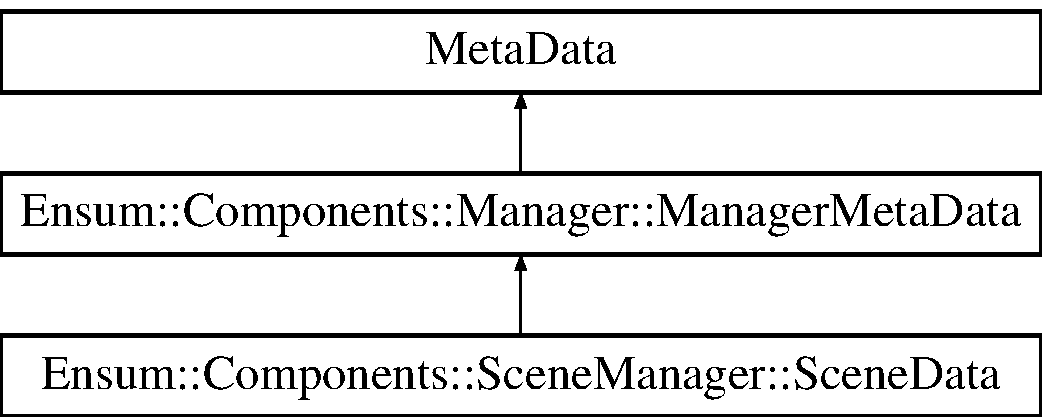
\includegraphics[height=3.000000cm]{struct_meta_data}
\end{center}
\end{figure}
\subsection*{Public Attributes}
\begin{DoxyCompactItemize}
\item 
uint32\+\_\+t {\bfseries used} = 0\hypertarget{struct_meta_data_abdcac78a4eaf9c6e69d4fdc0c0f1a1cf}{}\label{struct_meta_data_abdcac78a4eaf9c6e69d4fdc0c0f1a1cf}

\item 
uint32\+\_\+t {\bfseries allocated} = 0\hypertarget{struct_meta_data_ad7f915f404b7b1b3d46a19b0fa6f9a0c}{}\label{struct_meta_data_ad7f915f404b7b1b3d46a19b0fa6f9a0c}

\item 
void $\ast$ {\bfseries buffer} = nullptr\hypertarget{struct_meta_data_a3d09d759d39ddf22e23b3783d82b1c68}{}\label{struct_meta_data_a3d09d759d39ddf22e23b3783d82b1c68}

\end{DoxyCompactItemize}


The documentation for this struct was generated from the following file\+:\begin{DoxyCompactItemize}
\item 
C\+:/\+Users/peter/\+Source/\+Repos/\+E\+N\+S\+U\+M/\+Ensum/\+Includes/Data\+\_\+\+Meta.\+h\end{DoxyCompactItemize}

\hypertarget{class_ensum_1_1_components_1_1_null_scene}{}\section{Ensum\+:\+:Components\+:\+:Null\+Scene Class Reference}
\label{class_ensum_1_1_components_1_1_null_scene}\index{Ensum\+::\+Components\+::\+Null\+Scene@{Ensum\+::\+Components\+::\+Null\+Scene}}


A scene that does nothing.  




{\ttfamily \#include $<$Null\+Scene.\+h$>$}

Inheritance diagram for Ensum\+:\+:Components\+:\+:Null\+Scene\+:\begin{figure}[H]
\begin{center}
\leavevmode
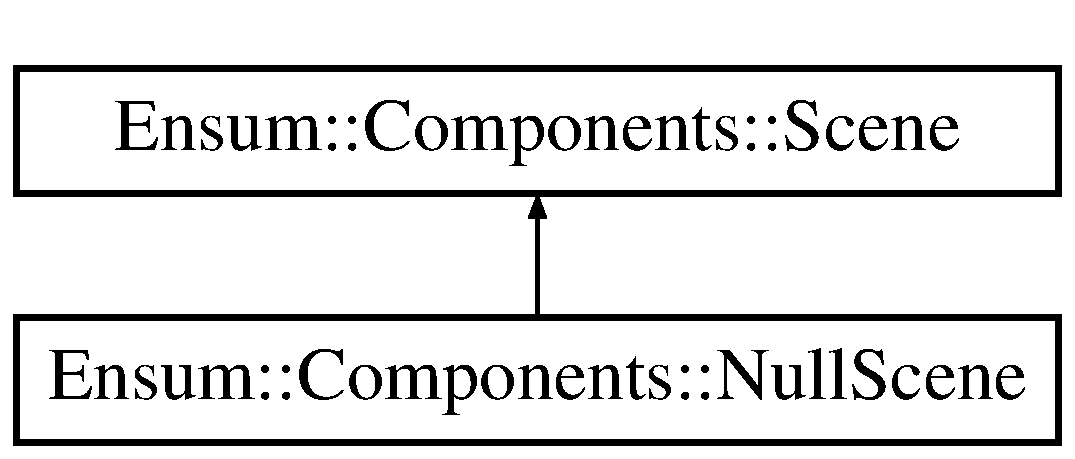
\includegraphics[height=2.000000cm]{class_ensum_1_1_components_1_1_null_scene}
\end{center}
\end{figure}
\subsection*{Public Member Functions}
\begin{DoxyCompactItemize}
\item 
{\bfseries Null\+Scene} (\hyperlink{class_ensum_1_1_components_1_1_entity_manager}{Entity\+Manager} \&entity\+Manger, \hyperlink{class_ensum_1_1_input_1_1_input}{Input\+::\+Input} $\ast$input)\hypertarget{class_ensum_1_1_components_1_1_null_scene_a140c16207aa1450a50a78bd4030cffb4}{}\label{class_ensum_1_1_components_1_1_null_scene_a140c16207aa1450a50a78bd4030cffb4}

\end{DoxyCompactItemize}
\subsection*{Additional Inherited Members}


\subsection{Detailed Description}
A scene that does nothing. 

The documentation for this class was generated from the following file\+:\begin{DoxyCompactItemize}
\item 
C\+:/\+Users/peter/\+Source/\+Repos/\+E\+N\+S\+U\+M/\+Ensum/\+Includes/\+Ensum\+\_\+components/Null\+Scene.\+h\end{DoxyCompactItemize}

\hypertarget{class_ensum_1_1_utils_1_1_options}{}\section{Ensum\+:\+:Utils\+:\+:Options Class Reference}
\label{class_ensum_1_1_utils_1_1_options}\index{Ensum\+::\+Utils\+::\+Options@{Ensum\+::\+Utils\+::\+Options}}


A singleton class for reading and writing to config file.  




{\ttfamily \#include $<$Options.\+h$>$}

\subsection*{Static Public Member Functions}
\begin{DoxyCompactItemize}
\item 
static E\+N\+S\+U\+M\+\_\+\+U\+T\+I\+L\+S\+\_\+\+E\+X\+P\+O\+RT void \hyperlink{class_ensum_1_1_utils_1_1_options_a42cd72b90a957177404071c01bca1ea0}{Create\+Instance} ()
\begin{DoxyCompactList}\small\item\em Create the options instance. \end{DoxyCompactList}\item 
static E\+N\+S\+U\+M\+\_\+\+U\+T\+I\+L\+S\+\_\+\+E\+X\+P\+O\+RT void \hyperlink{class_ensum_1_1_utils_1_1_options_ace3ea5450fca95ba36201463cb47c3da}{Delete\+Instance} ()\hypertarget{class_ensum_1_1_utils_1_1_options_ace3ea5450fca95ba36201463cb47c3da}{}\label{class_ensum_1_1_utils_1_1_options_ace3ea5450fca95ba36201463cb47c3da}

\begin{DoxyCompactList}\small\item\em Deletes the instance. \end{DoxyCompactList}\item 
static E\+N\+S\+U\+M\+\_\+\+U\+T\+I\+L\+S\+\_\+\+E\+X\+P\+O\+RT long \hyperlink{class_ensum_1_1_utils_1_1_options_a784e8e989bea701170af8b689f040e90}{Get\+Integer\+Option} (const \hyperlink{class_ensum_1_1string}{string} \&section, const \hyperlink{class_ensum_1_1string}{string} \&option, long default\+\_\+value)\hypertarget{class_ensum_1_1_utils_1_1_options_a784e8e989bea701170af8b689f040e90}{}\label{class_ensum_1_1_utils_1_1_options_a784e8e989bea701170af8b689f040e90}

\begin{DoxyCompactList}\small\item\em Public read function. \end{DoxyCompactList}\item 
static E\+N\+S\+U\+M\+\_\+\+U\+T\+I\+L\+S\+\_\+\+E\+X\+P\+O\+RT double \hyperlink{class_ensum_1_1_utils_1_1_options_ac57c333c1f9bd66472fecaa8b7f55f30}{Get\+Real\+Option} (const \hyperlink{class_ensum_1_1string}{string} \&section, const \hyperlink{class_ensum_1_1string}{string} \&option, double default\+\_\+value)\hypertarget{class_ensum_1_1_utils_1_1_options_ac57c333c1f9bd66472fecaa8b7f55f30}{}\label{class_ensum_1_1_utils_1_1_options_ac57c333c1f9bd66472fecaa8b7f55f30}

\begin{DoxyCompactList}\small\item\em Public read function. \end{DoxyCompactList}\item 
static E\+N\+S\+U\+M\+\_\+\+U\+T\+I\+L\+S\+\_\+\+E\+X\+P\+O\+RT bool \hyperlink{class_ensum_1_1_utils_1_1_options_ad0925b8894344c6d4425fbf0acde3852}{Get\+Boolean\+Option} (const \hyperlink{class_ensum_1_1string}{string} \&section, const \hyperlink{class_ensum_1_1string}{string} \&option, bool default\+\_\+value)\hypertarget{class_ensum_1_1_utils_1_1_options_ad0925b8894344c6d4425fbf0acde3852}{}\label{class_ensum_1_1_utils_1_1_options_ad0925b8894344c6d4425fbf0acde3852}

\begin{DoxyCompactList}\small\item\em Public read function. \end{DoxyCompactList}\item 
static E\+N\+S\+U\+M\+\_\+\+U\+T\+I\+L\+S\+\_\+\+E\+X\+P\+O\+RT \hyperlink{class_ensum_1_1string}{string} \hyperlink{class_ensum_1_1_utils_1_1_options_ac89c9d4c8e4dde0a1b07745c97d082a9}{Get\+String\+Option} (const \hyperlink{class_ensum_1_1string}{string} \&section, const \hyperlink{class_ensum_1_1string}{string} \&option, const \hyperlink{class_ensum_1_1string}{string} \&default\+\_\+value)\hypertarget{class_ensum_1_1_utils_1_1_options_ac89c9d4c8e4dde0a1b07745c97d082a9}{}\label{class_ensum_1_1_utils_1_1_options_ac89c9d4c8e4dde0a1b07745c97d082a9}

\begin{DoxyCompactList}\small\item\em Public read function. \end{DoxyCompactList}\item 
static E\+N\+S\+U\+M\+\_\+\+U\+T\+I\+L\+S\+\_\+\+E\+X\+P\+O\+RT void \hyperlink{class_ensum_1_1_utils_1_1_options_a1d69b78fe5f4072908f5b615cd1ee9b4}{Set\+Integer\+Option} (const \hyperlink{class_ensum_1_1string}{string} \&section, const \hyperlink{class_ensum_1_1string}{string} \&option, long value)\hypertarget{class_ensum_1_1_utils_1_1_options_a1d69b78fe5f4072908f5b615cd1ee9b4}{}\label{class_ensum_1_1_utils_1_1_options_a1d69b78fe5f4072908f5b615cd1ee9b4}

\begin{DoxyCompactList}\small\item\em Public write function. \end{DoxyCompactList}\item 
static E\+N\+S\+U\+M\+\_\+\+U\+T\+I\+L\+S\+\_\+\+E\+X\+P\+O\+RT void \hyperlink{class_ensum_1_1_utils_1_1_options_ad8ebf2ce046cc95530f787bf372e7fd2}{Set\+Real\+Option} (const \hyperlink{class_ensum_1_1string}{string} \&section, const \hyperlink{class_ensum_1_1string}{string} \&option, double value)\hypertarget{class_ensum_1_1_utils_1_1_options_ad8ebf2ce046cc95530f787bf372e7fd2}{}\label{class_ensum_1_1_utils_1_1_options_ad8ebf2ce046cc95530f787bf372e7fd2}

\begin{DoxyCompactList}\small\item\em Public write function. \end{DoxyCompactList}\item 
static E\+N\+S\+U\+M\+\_\+\+U\+T\+I\+L\+S\+\_\+\+E\+X\+P\+O\+RT void \hyperlink{class_ensum_1_1_utils_1_1_options_a68837babb89a589bc49180fd849b2c28}{Set\+Boolean\+Option} (const \hyperlink{class_ensum_1_1string}{string} \&section, const \hyperlink{class_ensum_1_1string}{string} \&option, bool value)\hypertarget{class_ensum_1_1_utils_1_1_options_a68837babb89a589bc49180fd849b2c28}{}\label{class_ensum_1_1_utils_1_1_options_a68837babb89a589bc49180fd849b2c28}

\begin{DoxyCompactList}\small\item\em Public write function. \end{DoxyCompactList}\item 
static E\+N\+S\+U\+M\+\_\+\+U\+T\+I\+L\+S\+\_\+\+E\+X\+P\+O\+RT void \hyperlink{class_ensum_1_1_utils_1_1_options_a67df741524fdcd73f377d3b65f9699c9}{Set\+String\+Option} (const \hyperlink{class_ensum_1_1string}{string} \&section, const \hyperlink{class_ensum_1_1string}{string} \&option, const \hyperlink{class_ensum_1_1string}{string} \&value)\hypertarget{class_ensum_1_1_utils_1_1_options_a67df741524fdcd73f377d3b65f9699c9}{}\label{class_ensum_1_1_utils_1_1_options_a67df741524fdcd73f377d3b65f9699c9}

\begin{DoxyCompactList}\small\item\em Public write function. \end{DoxyCompactList}\item 
static E\+N\+S\+U\+M\+\_\+\+U\+T\+I\+L\+S\+\_\+\+E\+X\+P\+O\+RT void \hyperlink{class_ensum_1_1_utils_1_1_options_ab567217a53d2ef200574271fa3c957b1}{Subscribe} (\hyperlink{class_ensum_1_1_delegate}{Delegate}$<$ void()$>$ \&dele)
\begin{DoxyCompactList}\small\item\em Subscribe to the Options\+Change event. \end{DoxyCompactList}\item 
static E\+N\+S\+U\+M\+\_\+\+U\+T\+I\+L\+S\+\_\+\+E\+X\+P\+O\+RT void \hyperlink{class_ensum_1_1_utils_1_1_options_ac8945e45a27cd51401779bd92ae44fb2}{Un\+Subscribe} (\hyperlink{class_ensum_1_1_delegate}{Delegate}$<$ void()$>$ \&dele)\hypertarget{class_ensum_1_1_utils_1_1_options_ac8945e45a27cd51401779bd92ae44fb2}{}\label{class_ensum_1_1_utils_1_1_options_ac8945e45a27cd51401779bd92ae44fb2}

\begin{DoxyCompactList}\small\item\em Un\+Subscribe to the Options\+Change event. \end{DoxyCompactList}\end{DoxyCompactItemize}
\subsection*{Private Member Functions}
\begin{DoxyCompactItemize}
\item 
long \hyperlink{class_ensum_1_1_utils_1_1_options_a69b79cff0d5ad861b9f2be3bb296648f}{\+\_\+\+Get\+Integer\+Option} (const \hyperlink{class_ensum_1_1string}{string} \&section, const \hyperlink{class_ensum_1_1string}{string} \&option, long default\+\_\+value)\hypertarget{class_ensum_1_1_utils_1_1_options_a69b79cff0d5ad861b9f2be3bb296648f}{}\label{class_ensum_1_1_utils_1_1_options_a69b79cff0d5ad861b9f2be3bb296648f}

\begin{DoxyCompactList}\small\item\em Private Read function. \end{DoxyCompactList}\item 
double \hyperlink{class_ensum_1_1_utils_1_1_options_a3d79094def64e9e7bdbbe1c4532458e1}{\+\_\+\+Get\+Real\+Option} (const \hyperlink{class_ensum_1_1string}{string} \&section, const \hyperlink{class_ensum_1_1string}{string} \&option, double default\+\_\+value)\hypertarget{class_ensum_1_1_utils_1_1_options_a3d79094def64e9e7bdbbe1c4532458e1}{}\label{class_ensum_1_1_utils_1_1_options_a3d79094def64e9e7bdbbe1c4532458e1}

\begin{DoxyCompactList}\small\item\em Private Read function. \end{DoxyCompactList}\item 
bool \hyperlink{class_ensum_1_1_utils_1_1_options_a8c9a977bf971aa38af289af707a46490}{\+\_\+\+Get\+Boolean\+Option} (const \hyperlink{class_ensum_1_1string}{string} \&section, const \hyperlink{class_ensum_1_1string}{string} \&option, bool default\+\_\+value)\hypertarget{class_ensum_1_1_utils_1_1_options_a8c9a977bf971aa38af289af707a46490}{}\label{class_ensum_1_1_utils_1_1_options_a8c9a977bf971aa38af289af707a46490}

\begin{DoxyCompactList}\small\item\em Private Read function. \end{DoxyCompactList}\item 
\hyperlink{class_ensum_1_1string}{string} \hyperlink{class_ensum_1_1_utils_1_1_options_a741ecb0fda0375aa961d57108435c239}{\+\_\+\+Get\+String\+Option} (const \hyperlink{class_ensum_1_1string}{string} \&section, const \hyperlink{class_ensum_1_1string}{string} \&option, const \hyperlink{class_ensum_1_1string}{string} \&default\+\_\+value)\hypertarget{class_ensum_1_1_utils_1_1_options_a741ecb0fda0375aa961d57108435c239}{}\label{class_ensum_1_1_utils_1_1_options_a741ecb0fda0375aa961d57108435c239}

\begin{DoxyCompactList}\small\item\em Private Read function. \end{DoxyCompactList}\item 
void \hyperlink{class_ensum_1_1_utils_1_1_options_a8ed2a91a05fbabe8e83916adea5b2b96}{\+\_\+\+Set\+Integer\+Option} (const \hyperlink{class_ensum_1_1string}{string} \&section, const \hyperlink{class_ensum_1_1string}{string} \&option, long value)\hypertarget{class_ensum_1_1_utils_1_1_options_a8ed2a91a05fbabe8e83916adea5b2b96}{}\label{class_ensum_1_1_utils_1_1_options_a8ed2a91a05fbabe8e83916adea5b2b96}

\begin{DoxyCompactList}\small\item\em Private write function. \end{DoxyCompactList}\item 
void \hyperlink{class_ensum_1_1_utils_1_1_options_a1e6721c6556806ea91df7739c63e9ba2}{\+\_\+\+Set\+Real\+Option} (const \hyperlink{class_ensum_1_1string}{string} \&section, const \hyperlink{class_ensum_1_1string}{string} \&option, double value)\hypertarget{class_ensum_1_1_utils_1_1_options_a1e6721c6556806ea91df7739c63e9ba2}{}\label{class_ensum_1_1_utils_1_1_options_a1e6721c6556806ea91df7739c63e9ba2}

\begin{DoxyCompactList}\small\item\em Private write function. \end{DoxyCompactList}\item 
void \hyperlink{class_ensum_1_1_utils_1_1_options_ae7f2dc1a114d67fbe049454f6bb1aa1e}{\+\_\+\+Set\+Boolean\+Option} (const \hyperlink{class_ensum_1_1string}{string} \&section, const \hyperlink{class_ensum_1_1string}{string} \&option, bool value)\hypertarget{class_ensum_1_1_utils_1_1_options_ae7f2dc1a114d67fbe049454f6bb1aa1e}{}\label{class_ensum_1_1_utils_1_1_options_ae7f2dc1a114d67fbe049454f6bb1aa1e}

\begin{DoxyCompactList}\small\item\em Private write function. \end{DoxyCompactList}\item 
void \hyperlink{class_ensum_1_1_utils_1_1_options_a7ba0b31a187c20ffec4725b5f1fd9003}{\+\_\+\+Set\+String\+Option} (const \hyperlink{class_ensum_1_1string}{string} \&section, const \hyperlink{class_ensum_1_1string}{string} \&option, const \hyperlink{class_ensum_1_1string}{string} \&value)\hypertarget{class_ensum_1_1_utils_1_1_options_a7ba0b31a187c20ffec4725b5f1fd9003}{}\label{class_ensum_1_1_utils_1_1_options_a7ba0b31a187c20ffec4725b5f1fd9003}

\begin{DoxyCompactList}\small\item\em Private write function. \end{DoxyCompactList}\end{DoxyCompactItemize}
\subsection*{Private Attributes}
\begin{DoxyCompactItemize}
\item 
\hyperlink{class_ensum_1_1_file_handler_1_1ini}{File\+Handler\+::ini} $\ast$ {\bfseries \+\_\+file}\hypertarget{class_ensum_1_1_utils_1_1_options_ae10dba8ac3cb72c83e206ba2b74fa9c3}{}\label{class_ensum_1_1_utils_1_1_options_ae10dba8ac3cb72c83e206ba2b74fa9c3}

\item 
\hyperlink{class_ensum_1_1_event}{Event}$<$ void()$>$ {\bfseries \+\_\+\+Option\+Change}\hypertarget{class_ensum_1_1_utils_1_1_options_a8387d551a3972a8c09097fdc7b35c057}{}\label{class_ensum_1_1_utils_1_1_options_a8387d551a3972a8c09097fdc7b35c057}

\end{DoxyCompactItemize}
\subsection*{Static Private Attributes}
\begin{DoxyCompactItemize}
\item 
static \hyperlink{class_ensum_1_1_utils_1_1_options}{Options} $\ast$ {\bfseries \+\_\+instance}\hypertarget{class_ensum_1_1_utils_1_1_options_ade4681c12beae9f1acd240c4bdc2fb21}{}\label{class_ensum_1_1_utils_1_1_options_ade4681c12beae9f1acd240c4bdc2fb21}

\end{DoxyCompactItemize}


\subsection{Detailed Description}
A singleton class for reading and writing to config file. 

\subsection{Member Function Documentation}
\index{Ensum\+::\+Utils\+::\+Options@{Ensum\+::\+Utils\+::\+Options}!Create\+Instance@{Create\+Instance}}
\index{Create\+Instance@{Create\+Instance}!Ensum\+::\+Utils\+::\+Options@{Ensum\+::\+Utils\+::\+Options}}
\subsubsection[{\texorpdfstring{Create\+Instance()}{CreateInstance()}}]{\setlength{\rightskip}{0pt plus 5cm}static E\+N\+S\+U\+M\+\_\+\+U\+T\+I\+L\+S\+\_\+\+E\+X\+P\+O\+RT void Ensum\+::\+Utils\+::\+Options\+::\+Create\+Instance (
\begin{DoxyParamCaption}
{}
\end{DoxyParamCaption}
)\hspace{0.3cm}{\ttfamily [static]}}\hypertarget{class_ensum_1_1_utils_1_1_options_a42cd72b90a957177404071c01bca1ea0}{}\label{class_ensum_1_1_utils_1_1_options_a42cd72b90a957177404071c01bca1ea0}


Create the options instance. 

If options are not used all clients will simply use default values. \index{Ensum\+::\+Utils\+::\+Options@{Ensum\+::\+Utils\+::\+Options}!Subscribe@{Subscribe}}
\index{Subscribe@{Subscribe}!Ensum\+::\+Utils\+::\+Options@{Ensum\+::\+Utils\+::\+Options}}
\subsubsection[{\texorpdfstring{Subscribe(\+Delegate$<$ void()$>$ \&dele)}{Subscribe(Delegate< void()> &dele)}}]{\setlength{\rightskip}{0pt plus 5cm}static E\+N\+S\+U\+M\+\_\+\+U\+T\+I\+L\+S\+\_\+\+E\+X\+P\+O\+RT void Ensum\+::\+Utils\+::\+Options\+::\+Subscribe (
\begin{DoxyParamCaption}
\item[{{\bf Delegate}$<$ void()$>$ \&}]{dele}
\end{DoxyParamCaption}
)\hspace{0.3cm}{\ttfamily [static]}}\hypertarget{class_ensum_1_1_utils_1_1_options_ab567217a53d2ef200574271fa3c957b1}{}\label{class_ensum_1_1_utils_1_1_options_ab567217a53d2ef200574271fa3c957b1}


Subscribe to the Options\+Change event. 

When a change occurs in options this event is called. 

The documentation for this class was generated from the following file\+:\begin{DoxyCompactItemize}
\item 
Includes/\+Ensum\+\_\+utils/Options.\+h\end{DoxyCompactItemize}

\hypertarget{class_ensum_1_1_components_1_1_scene}{}\section{Ensum\+:\+:Components\+:\+:Scene Class Reference}
\label{class_ensum_1_1_components_1_1_scene}\index{Ensum\+::\+Components\+::\+Scene@{Ensum\+::\+Components\+::\+Scene}}


The abstract scene class.  




{\ttfamily \#include $<$Scene.\+h$>$}

Inheritance diagram for Ensum\+:\+:Components\+:\+:Scene\+:\begin{figure}[H]
\begin{center}
\leavevmode
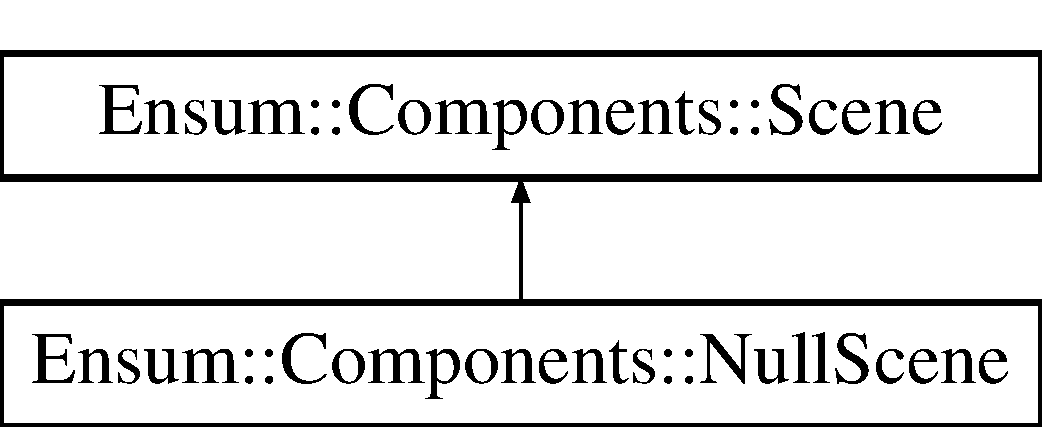
\includegraphics[height=2.000000cm]{class_ensum_1_1_components_1_1_scene}
\end{center}
\end{figure}
\subsection*{Public Member Functions}
\begin{DoxyCompactItemize}
\item 
virtual const \hyperlink{struct_ensum_1_1_components_1_1_entity}{Entity} \& \hyperlink{class_ensum_1_1_components_1_1_scene_ab614d491401edd9db3584d4e61ef6416}{Get\+Entity} () const \hypertarget{class_ensum_1_1_components_1_1_scene_ab614d491401edd9db3584d4e61ef6416}{}\label{class_ensum_1_1_components_1_1_scene_ab614d491401edd9db3584d4e61ef6416}

\begin{DoxyCompactList}\small\item\em Returns the scenes entity. \end{DoxyCompactList}\item 
virtual const void \hyperlink{class_ensum_1_1_components_1_1_scene_a4f12d73cbbd3e203bfc60eac07318985}{Frame} ()\hypertarget{class_ensum_1_1_components_1_1_scene_a4f12d73cbbd3e203bfc60eac07318985}{}\label{class_ensum_1_1_components_1_1_scene_a4f12d73cbbd3e203bfc60eac07318985}

\begin{DoxyCompactList}\small\item\em The frame function for the scene. \end{DoxyCompactList}\end{DoxyCompactItemize}
\subsection*{Protected Member Functions}
\begin{DoxyCompactItemize}
\item 
{\bfseries Scene} (\hyperlink{class_ensum_1_1_components_1_1_entity_manager}{Entity\+Manager} \&entity\+Manger, \hyperlink{class_ensum_1_1_input_1_1_input}{Input\+::\+Input} $\ast$input)\hypertarget{class_ensum_1_1_components_1_1_scene_aee190492d4435b67533941958ff81a8e}{}\label{class_ensum_1_1_components_1_1_scene_aee190492d4435b67533941958ff81a8e}

\end{DoxyCompactItemize}
\subsection*{Protected Attributes}
\begin{DoxyCompactItemize}
\item 
\hyperlink{struct_ensum_1_1_components_1_1_entity}{Entity} \hyperlink{class_ensum_1_1_components_1_1_scene_a8d36e81874a5b07e3edbd8720b8b289e}{\+\_\+entity}
\item 
\hyperlink{class_ensum_1_1_components_1_1_entity_manager}{Entity\+Manager} \& \hyperlink{class_ensum_1_1_components_1_1_scene_af7eb8e3279c5b6768f442ae05b44e75f}{\+\_\+entity\+Manager}
\item 
\hyperlink{class_ensum_1_1_input_1_1_input}{Input\+::\+Input} $\ast$ {\bfseries \+\_\+input}\hypertarget{class_ensum_1_1_components_1_1_scene_ab7ee39773379321c85d73984b03c5568}{}\label{class_ensum_1_1_components_1_1_scene_ab7ee39773379321c85d73984b03c5568}

\item 
std\+::vector$<$ \hyperlink{class_ensum_1_1_components_1_1_manager}{Manager} $\ast$ $>$ $\ast$ \hyperlink{class_ensum_1_1_components_1_1_scene_a9f7c53f74805c8bf7461f9ff2c818be7}{\+\_\+managers}
\begin{DoxyCompactList}\small\item\em Create new instance of all other managers here. \end{DoxyCompactList}\item 
\hyperlink{class_ensum_1_1_components_1_1_data_manager}{Data\+Manager} {\bfseries \+\_\+data}\hypertarget{class_ensum_1_1_components_1_1_scene_ae6357dc18aece3e778ce642f59f8195b}{}\label{class_ensum_1_1_components_1_1_scene_ae6357dc18aece3e778ce642f59f8195b}

\item 
\hyperlink{class_ensum_1_1_components_1_1_transform_manager}{Transform\+Manager} {\bfseries \+\_\+transform}\hypertarget{class_ensum_1_1_components_1_1_scene_a9f8a3149409a891d77b5554c154deb65}{}\label{class_ensum_1_1_components_1_1_scene_a9f8a3149409a891d77b5554c154deb65}

\item 
\hyperlink{class_ensum_1_1_components_1_1_camera_manager}{Camera\+Manager} {\bfseries \+\_\+camera}\hypertarget{class_ensum_1_1_components_1_1_scene_a9d4a91f7879f6392a6d95dfeea6608a2}{}\label{class_ensum_1_1_components_1_1_scene_a9d4a91f7879f6392a6d95dfeea6608a2}

\item 
\hyperlink{class_ensum_1_1_components_1_1_static_mesh_manager}{Static\+Mesh\+Manager} {\bfseries \+\_\+static\+Meshes}\hypertarget{class_ensum_1_1_components_1_1_scene_a790b65abe3f86eae4e082a4557fc07d8}{}\label{class_ensum_1_1_components_1_1_scene_a790b65abe3f86eae4e082a4557fc07d8}

\end{DoxyCompactItemize}


\subsection{Detailed Description}
The abstract scene class. 

A scene could be considered it\textquotesingle{}s own world or a state in a statemachine. 

\subsection{Member Data Documentation}
\index{Ensum\+::\+Components\+::\+Scene@{Ensum\+::\+Components\+::\+Scene}!\+\_\+entity@{\+\_\+entity}}
\index{\+\_\+entity@{\+\_\+entity}!Ensum\+::\+Components\+::\+Scene@{Ensum\+::\+Components\+::\+Scene}}
\subsubsection[{\texorpdfstring{\+\_\+entity}{_entity}}]{\setlength{\rightskip}{0pt plus 5cm}{\bf Entity} Ensum\+::\+Components\+::\+Scene\+::\+\_\+entity\hspace{0.3cm}{\ttfamily [protected]}}\hypertarget{class_ensum_1_1_components_1_1_scene_a8d36e81874a5b07e3edbd8720b8b289e}{}\label{class_ensum_1_1_components_1_1_scene_a8d36e81874a5b07e3edbd8720b8b289e}
The scenes own entity \index{Ensum\+::\+Components\+::\+Scene@{Ensum\+::\+Components\+::\+Scene}!\+\_\+entity\+Manager@{\+\_\+entity\+Manager}}
\index{\+\_\+entity\+Manager@{\+\_\+entity\+Manager}!Ensum\+::\+Components\+::\+Scene@{Ensum\+::\+Components\+::\+Scene}}
\subsubsection[{\texorpdfstring{\+\_\+entity\+Manager}{_entityManager}}]{\setlength{\rightskip}{0pt plus 5cm}{\bf Entity\+Manager}\& Ensum\+::\+Components\+::\+Scene\+::\+\_\+entity\+Manager\hspace{0.3cm}{\ttfamily [protected]}}\hypertarget{class_ensum_1_1_components_1_1_scene_af7eb8e3279c5b6768f442ae05b44e75f}{}\label{class_ensum_1_1_components_1_1_scene_af7eb8e3279c5b6768f442ae05b44e75f}
A reference to the entitymanager created in scenemanager \index{Ensum\+::\+Components\+::\+Scene@{Ensum\+::\+Components\+::\+Scene}!\+\_\+managers@{\+\_\+managers}}
\index{\+\_\+managers@{\+\_\+managers}!Ensum\+::\+Components\+::\+Scene@{Ensum\+::\+Components\+::\+Scene}}
\subsubsection[{\texorpdfstring{\+\_\+managers}{_managers}}]{\setlength{\rightskip}{0pt plus 5cm}std\+::vector$<${\bf Manager}$\ast$$>$$\ast$ Ensum\+::\+Components\+::\+Scene\+::\+\_\+managers\hspace{0.3cm}{\ttfamily [protected]}}\hypertarget{class_ensum_1_1_components_1_1_scene_a9f7c53f74805c8bf7461f9ff2c818be7}{}\label{class_ensum_1_1_components_1_1_scene_a9f7c53f74805c8bf7461f9ff2c818be7}


Create new instance of all other managers here. 

Every new manager needs to be initiated in the constructor and added to the managers vector. 

The documentation for this class was generated from the following file\+:\begin{DoxyCompactItemize}
\item 
C\+:/\+Users/peter/\+Source/\+Repos/\+E\+N\+S\+U\+M/\+Ensum/\+Includes/\+Ensum\+\_\+components/Scene.\+h\end{DoxyCompactItemize}

\hypertarget{struct_ensum_1_1_components_1_1_scene_manager_1_1_scene_data}{}\section{Ensum\+:\+:Components\+:\+:Scene\+Manager\+:\+:Scene\+Data Struct Reference}
\label{struct_ensum_1_1_components_1_1_scene_manager_1_1_scene_data}\index{Ensum\+::\+Components\+::\+Scene\+Manager\+::\+Scene\+Data@{Ensum\+::\+Components\+::\+Scene\+Manager\+::\+Scene\+Data}}
\subsection*{Public Attributes}
\begin{DoxyCompactItemize}
\item 
\hyperlink{struct_meta_data}{Meta\+Data} {\bfseries meta}\hypertarget{struct_ensum_1_1_components_1_1_scene_manager_1_1_scene_data_a86f40c9cb2aa13ae41ee7521dcf416cc}{}\label{struct_ensum_1_1_components_1_1_scene_manager_1_1_scene_data_a86f40c9cb2aa13ae41ee7521dcf416cc}

\item 
\hyperlink{struct_ensum_1_1_components_1_1_entity}{Entity} $\ast$ {\bfseries entity}\hypertarget{struct_ensum_1_1_components_1_1_scene_manager_1_1_scene_data_aff477aef5752b1b0f438ef0e986a9229}{}\label{struct_ensum_1_1_components_1_1_scene_manager_1_1_scene_data_aff477aef5752b1b0f438ef0e986a9229}

\item 
\hyperlink{class_ensum_1_1_components_1_1_scene}{Scene} $\ast$$\ast$ {\bfseries scene\+Ptr}\hypertarget{struct_ensum_1_1_components_1_1_scene_manager_1_1_scene_data_ac37964615c53887051adcc587fa9dab0}{}\label{struct_ensum_1_1_components_1_1_scene_manager_1_1_scene_data_ac37964615c53887051adcc587fa9dab0}

\item 
bool $\ast$ {\bfseries scene\+Update}\hypertarget{struct_ensum_1_1_components_1_1_scene_manager_1_1_scene_data_a7d4a9e3d7aed5dc8f338b4d4a312f875}{}\label{struct_ensum_1_1_components_1_1_scene_manager_1_1_scene_data_a7d4a9e3d7aed5dc8f338b4d4a312f875}

\end{DoxyCompactItemize}


The documentation for this struct was generated from the following file\+:\begin{DoxyCompactItemize}
\item 
Includes/\+Ensum\+\_\+components/Scene\+Manager.\+h\end{DoxyCompactItemize}

\hypertarget{class_ensum_1_1_components_1_1_scene_manager}{}\section{Ensum\+:\+:Components\+:\+:Scene\+Manager Class Reference}
\label{class_ensum_1_1_components_1_1_scene_manager}\index{Ensum\+::\+Components\+::\+Scene\+Manager@{Ensum\+::\+Components\+::\+Scene\+Manager}}


Manages all the scenes.  




{\ttfamily \#include $<$Scene\+Manager.\+h$>$}

Inheritance diagram for Ensum\+:\+:Components\+:\+:Scene\+Manager\+:\begin{figure}[H]
\begin{center}
\leavevmode
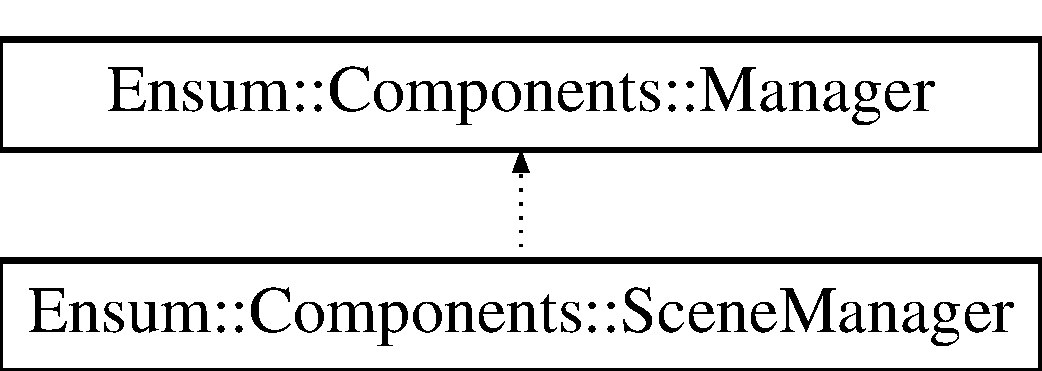
\includegraphics[height=2.000000cm]{class_ensum_1_1_components_1_1_scene_manager}
\end{center}
\end{figure}
\subsection*{Classes}
\begin{DoxyCompactItemize}
\item 
struct \hyperlink{struct_ensum_1_1_components_1_1_scene_manager_1_1_scene_data}{Scene\+Data}
\end{DoxyCompactItemize}
\subsection*{Public Member Functions}
\begin{DoxyCompactItemize}
\item 
const \hyperlink{struct_ensum_1_1_components_1_1_entity}{Entity} \& \hyperlink{class_ensum_1_1_components_1_1_scene_manager_a4a71bb9192da118a71f1b81ca49742cb}{Create\+Scene} (\hyperlink{class_ensum_1_1_components_1_1_scene}{Scene} $\ast$scene)\hypertarget{class_ensum_1_1_components_1_1_scene_manager_a4a71bb9192da118a71f1b81ca49742cb}{}\label{class_ensum_1_1_components_1_1_scene_manager_a4a71bb9192da118a71f1b81ca49742cb}

\begin{DoxyCompactList}\small\item\em Create the scene and return it\textquotesingle{}s entity. \end{DoxyCompactList}\item 
const void \hyperlink{class_ensum_1_1_components_1_1_scene_manager_ab970d3716b08c39b9b8c5484dea11595}{Remove\+Scene} (const \hyperlink{struct_ensum_1_1_components_1_1_entity}{Entity} \&scene\+Entity)\hypertarget{class_ensum_1_1_components_1_1_scene_manager_ab970d3716b08c39b9b8c5484dea11595}{}\label{class_ensum_1_1_components_1_1_scene_manager_ab970d3716b08c39b9b8c5484dea11595}

\begin{DoxyCompactList}\small\item\em Remove the scene component from the entity. \end{DoxyCompactList}\item 
const void \hyperlink{class_ensum_1_1_components_1_1_scene_manager_aea9f13488931b4448778e5563685428e}{Set\+Update} (const \hyperlink{struct_ensum_1_1_components_1_1_entity}{Entity} \&scene\+Entity, bool update)\hypertarget{class_ensum_1_1_components_1_1_scene_manager_aea9f13488931b4448778e5563685428e}{}\label{class_ensum_1_1_components_1_1_scene_manager_aea9f13488931b4448778e5563685428e}

\begin{DoxyCompactList}\small\item\em Specifies whether the scene should be updated each frame. \end{DoxyCompactList}\item 
const void \hyperlink{class_ensum_1_1_components_1_1_scene_manager_ad33a35aa27eeae297a4f16c610205d8a}{Frame} ()\hypertarget{class_ensum_1_1_components_1_1_scene_manager_ad33a35aa27eeae297a4f16c610205d8a}{}\label{class_ensum_1_1_components_1_1_scene_manager_ad33a35aa27eeae297a4f16c610205d8a}

\begin{DoxyCompactList}\small\item\em Do the framework for all active scenes. \end{DoxyCompactList}\item 
\hyperlink{class_ensum_1_1_components_1_1_entity_manager}{Entity\+Manager} \& \hyperlink{class_ensum_1_1_components_1_1_scene_manager_a7fdc5d47c5b8fe03807fe472b038a56f}{Get\+Entity\+Manager} ()\hypertarget{class_ensum_1_1_components_1_1_scene_manager_a7fdc5d47c5b8fe03807fe472b038a56f}{}\label{class_ensum_1_1_components_1_1_scene_manager_a7fdc5d47c5b8fe03807fe472b038a56f}

\begin{DoxyCompactList}\small\item\em Return a reference to the entity manager. \end{DoxyCompactList}\end{DoxyCompactItemize}
\subsection*{Private Member Functions}
\begin{DoxyCompactItemize}
\item 
const void \hyperlink{class_ensum_1_1_components_1_1_scene_manager_a383a468319c93280ce8ac0bbb920ab87}{\+\_\+\+Allocate} (uint32\+\_\+t size)
\begin{DoxyCompactList}\small\item\em Allocate more memory for scenedata. \end{DoxyCompactList}\item 
const void \hyperlink{class_ensum_1_1_components_1_1_scene_manager_a8102cfd9f4fed62a06e564dc016b6c46}{\+\_\+\+Destroy} (uint32\+\_\+t index)
\begin{DoxyCompactList}\small\item\em Delete an entry in the memory block. \end{DoxyCompactList}\end{DoxyCompactItemize}
\subsection*{Private Attributes}
\begin{DoxyCompactItemize}
\item 
\hyperlink{class_ensum_1_1_components_1_1_entity_manager}{Entity\+Manager} \hyperlink{class_ensum_1_1_components_1_1_scene_manager_a1be3bed380d7f6712e9c6c3bb71c048a}{\+\_\+ent\+Manager}\hypertarget{class_ensum_1_1_components_1_1_scene_manager_a1be3bed380d7f6712e9c6c3bb71c048a}{}\label{class_ensum_1_1_components_1_1_scene_manager_a1be3bed380d7f6712e9c6c3bb71c048a}

\begin{DoxyCompactList}\small\item\em Looks for destroyed entities and deletes them from the data block. \end{DoxyCompactList}\item 
\hyperlink{class_ensum_1_1_input_1_1_input}{Input\+::\+Input} $\ast$ {\bfseries \+\_\+input}\hypertarget{class_ensum_1_1_components_1_1_scene_manager_a997e4d367f66c9f80d27e027999f6802}{}\label{class_ensum_1_1_components_1_1_scene_manager_a997e4d367f66c9f80d27e027999f6802}

\item 
\hyperlink{struct_ensum_1_1_components_1_1_scene_manager_1_1_scene_data}{Scene\+Data} $\ast$ {\bfseries \+\_\+datap}\hypertarget{class_ensum_1_1_components_1_1_scene_manager_a249b282fedd2971d521e5a4a8922ceeb}{}\label{class_ensum_1_1_components_1_1_scene_manager_a249b282fedd2971d521e5a4a8922ceeb}

\end{DoxyCompactItemize}


\subsection{Detailed Description}
Manages all the scenes. 

\subsection{Member Function Documentation}
\index{Ensum\+::\+Components\+::\+Scene\+Manager@{Ensum\+::\+Components\+::\+Scene\+Manager}!\+\_\+\+Allocate@{\+\_\+\+Allocate}}
\index{\+\_\+\+Allocate@{\+\_\+\+Allocate}!Ensum\+::\+Components\+::\+Scene\+Manager@{Ensum\+::\+Components\+::\+Scene\+Manager}}
\subsubsection[{\texorpdfstring{\+\_\+\+Allocate(uint32\+\_\+t size)}{_Allocate(uint32_t size)}}]{\setlength{\rightskip}{0pt plus 5cm}const void Ensum\+::\+Components\+::\+Scene\+Manager\+::\+\_\+\+Allocate (
\begin{DoxyParamCaption}
\item[{uint32\+\_\+t}]{size}
\end{DoxyParamCaption}
)\hspace{0.3cm}{\ttfamily [private]}, {\ttfamily [virtual]}}\hypertarget{class_ensum_1_1_components_1_1_scene_manager_a383a468319c93280ce8ac0bbb920ab87}{}\label{class_ensum_1_1_components_1_1_scene_manager_a383a468319c93280ce8ac0bbb920ab87}


Allocate more memory for scenedata. 



Implements \hyperlink{class_ensum_1_1_components_1_1_manager_a1b593059210d09632c910a6abaae49c0}{Ensum\+::\+Components\+::\+Manager}.

\index{Ensum\+::\+Components\+::\+Scene\+Manager@{Ensum\+::\+Components\+::\+Scene\+Manager}!\+\_\+\+Destroy@{\+\_\+\+Destroy}}
\index{\+\_\+\+Destroy@{\+\_\+\+Destroy}!Ensum\+::\+Components\+::\+Scene\+Manager@{Ensum\+::\+Components\+::\+Scene\+Manager}}
\subsubsection[{\texorpdfstring{\+\_\+\+Destroy(uint32\+\_\+t index)}{_Destroy(uint32_t index)}}]{\setlength{\rightskip}{0pt plus 5cm}const void Ensum\+::\+Components\+::\+Scene\+Manager\+::\+\_\+\+Destroy (
\begin{DoxyParamCaption}
\item[{uint32\+\_\+t}]{index}
\end{DoxyParamCaption}
)\hspace{0.3cm}{\ttfamily [private]}, {\ttfamily [virtual]}}\hypertarget{class_ensum_1_1_components_1_1_scene_manager_a8102cfd9f4fed62a06e564dc016b6c46}{}\label{class_ensum_1_1_components_1_1_scene_manager_a8102cfd9f4fed62a06e564dc016b6c46}


Delete an entry in the memory block. 

The deleted entry is replaced by the last in the block. 

Implements \hyperlink{class_ensum_1_1_components_1_1_manager_a5ba85395802e942ed8904ca18951e6b0}{Ensum\+::\+Components\+::\+Manager}.



The documentation for this class was generated from the following file\+:\begin{DoxyCompactItemize}
\item 
C\+:/\+Users/peter/\+Source/\+Repos/\+E\+N\+S\+U\+M/\+Ensum/\+Includes/\+Ensum\+\_\+components/Scene\+Manager.\+h\end{DoxyCompactItemize}

\hypertarget{struct_ensum_1_1_file_handler_1_1ini_1_1_section}{}\section{Ensum\+:\+:File\+Handler\+:\+:ini\+:\+:Section Struct Reference}
\label{struct_ensum_1_1_file_handler_1_1ini_1_1_section}\index{Ensum\+::\+File\+Handler\+::ini\+::\+Section@{Ensum\+::\+File\+Handler\+::ini\+::\+Section}}
\subsection*{Public Member Functions}
\begin{DoxyCompactItemize}
\item 
{\bfseries Section} (const \hyperlink{class_ensum_1_1string}{string} \&sname)\hypertarget{struct_ensum_1_1_file_handler_1_1ini_1_1_section_aece352bd19575c13a3359ee2a16f375d}{}\label{struct_ensum_1_1_file_handler_1_1ini_1_1_section_aece352bd19575c13a3359ee2a16f375d}

\end{DoxyCompactItemize}
\subsection*{Public Attributes}
\begin{DoxyCompactItemize}
\item 
\hyperlink{class_ensum_1_1string}{string} {\bfseries name}\hypertarget{struct_ensum_1_1_file_handler_1_1ini_1_1_section_aaef5921ebec35dfe6b7ac00cde2e71a6}{}\label{struct_ensum_1_1_file_handler_1_1ini_1_1_section_aaef5921ebec35dfe6b7ac00cde2e71a6}

\item 
std\+::vector$<$ \hyperlink{struct_ensum_1_1_file_handler_1_1ini_1_1_key}{Key} $>$ {\bfseries keys}\hypertarget{struct_ensum_1_1_file_handler_1_1ini_1_1_section_a4ef77125d407902a380c30d3f0f120da}{}\label{struct_ensum_1_1_file_handler_1_1ini_1_1_section_a4ef77125d407902a380c30d3f0f120da}

\end{DoxyCompactItemize}


The documentation for this struct was generated from the following file\+:\begin{DoxyCompactItemize}
\item 
Includes/\+Ensum\+\_\+filehandler/Ini.\+h\end{DoxyCompactItemize}

\hypertarget{class_ensum_1_1string}{}\section{Ensum\+:\+:string Class Reference}
\label{class_ensum_1_1string}\index{Ensum\+::string@{Ensum\+::string}}


A wrapper class for std\+::string.  




{\ttfamily \#include $<$ensumstring.\+h$>$}

\subsection*{Public Member Functions}
\begin{DoxyCompactItemize}
\item 
{\bfseries string} (const char $\ast$str)\hypertarget{class_ensum_1_1string_a1efde732b942cf5b4a9aeff02836c7f4}{}\label{class_ensum_1_1string_a1efde732b942cf5b4a9aeff02836c7f4}

\item 
{\bfseries string} (const \hyperlink{class_ensum_1_1string}{string} \&other)\hypertarget{class_ensum_1_1string_a941a6aeb4f7e6f8a61a375a19ada9e36}{}\label{class_ensum_1_1string_a941a6aeb4f7e6f8a61a375a19ada9e36}

\item 
{\bfseries string} (const long \&other)\hypertarget{class_ensum_1_1string_ab94e9717ef713acd5981ad9d2c9d0a5e}{}\label{class_ensum_1_1string_ab94e9717ef713acd5981ad9d2c9d0a5e}

\item 
{\bfseries string} (const double \&other)\hypertarget{class_ensum_1_1string_ad2d7d12b303783eb4ecc32a389e1c42b}{}\label{class_ensum_1_1string_ad2d7d12b303783eb4ecc32a389e1c42b}

\item 
{\bfseries string} (const bool \&other)\hypertarget{class_ensum_1_1string_a82ccf9bec24664a575b8e9c70cbd7d99}{}\label{class_ensum_1_1string_a82ccf9bec24664a575b8e9c70cbd7d99}

\item 
\hyperlink{class_ensum_1_1string}{string} \hyperlink{class_ensum_1_1string_a13098a5e0f0fd18baeffa5bc8b35494d}{operator+} (const \hyperlink{class_ensum_1_1string}{string} \&str) const 
\item 
\hyperlink{class_ensum_1_1string}{string} \hyperlink{class_ensum_1_1string_aa9f884ae697a27d375d6dc71fd5a1602}{operator+} (const char $\ast$str) const 
\item 
\hyperlink{class_ensum_1_1string_ae1473c4afee1fb83de48490a72f8266b}{operator const char $\ast$} () const \hypertarget{class_ensum_1_1string_ae1473c4afee1fb83de48490a72f8266b}{}\label{class_ensum_1_1string_ae1473c4afee1fb83de48490a72f8266b}

\begin{DoxyCompactList}\small\item\em convertion operator to char$\ast$. \end{DoxyCompactList}\item 
\hyperlink{class_ensum_1_1string_a6fa9ce4490f285575c2d06a1e64a93a7}{operator const void $\ast$} () const \hypertarget{class_ensum_1_1string_a6fa9ce4490f285575c2d06a1e64a93a7}{}\label{class_ensum_1_1string_a6fa9ce4490f285575c2d06a1e64a93a7}

\begin{DoxyCompactList}\small\item\em convertion operator to void$\ast$. \end{DoxyCompactList}\item 
\hyperlink{class_ensum_1_1string}{string} \& \hyperlink{class_ensum_1_1string_ae48b8f643d8cd3ff379a51484ea738d1}{operator=} (const char $\ast$str)\hypertarget{class_ensum_1_1string_ae48b8f643d8cd3ff379a51484ea738d1}{}\label{class_ensum_1_1string_ae48b8f643d8cd3ff379a51484ea738d1}

\begin{DoxyCompactList}\small\item\em = operator char. \end{DoxyCompactList}\item 
\hyperlink{class_ensum_1_1string}{string} \& \hyperlink{class_ensum_1_1string_a7903e871b1cf12584d746536241fa7ea}{operator=} (const \hyperlink{class_ensum_1_1string}{string} \&other)\hypertarget{class_ensum_1_1string_a7903e871b1cf12584d746536241fa7ea}{}\label{class_ensum_1_1string_a7903e871b1cf12584d746536241fa7ea}

\begin{DoxyCompactList}\small\item\em = operator string. \end{DoxyCompactList}\item 
const bool \hyperlink{class_ensum_1_1string_a6b5ab08eb5ef197bedb9e55e2eca0754}{operator==} (const char $\ast$str)\hypertarget{class_ensum_1_1string_a6b5ab08eb5ef197bedb9e55e2eca0754}{}\label{class_ensum_1_1string_a6b5ab08eb5ef197bedb9e55e2eca0754}

\begin{DoxyCompactList}\small\item\em == operator char. \end{DoxyCompactList}\item 
const bool \hyperlink{class_ensum_1_1string_a6429683caad1908c30cb77b4aa00ff4f}{operator==} (const \hyperlink{class_ensum_1_1string}{string} \&other)\hypertarget{class_ensum_1_1string_a6429683caad1908c30cb77b4aa00ff4f}{}\label{class_ensum_1_1string_a6429683caad1908c30cb77b4aa00ff4f}

\begin{DoxyCompactList}\small\item\em == operator string. \end{DoxyCompactList}\item 
const char $\ast$ \hyperlink{class_ensum_1_1string_a2d667ea4adbf4f9cd08011972176aacb}{c\+\_\+str} () const \hypertarget{class_ensum_1_1string_a2d667ea4adbf4f9cd08011972176aacb}{}\label{class_ensum_1_1string_a2d667ea4adbf4f9cd08011972176aacb}

\begin{DoxyCompactList}\small\item\em returns const char$\ast$. \end{DoxyCompactList}\item 
const void \hyperlink{class_ensum_1_1string_ad183e0697bed62d8e5639d17a5288a15}{transform} ()\hypertarget{class_ensum_1_1string_ad183e0697bed62d8e5639d17a5288a15}{}\label{class_ensum_1_1string_ad183e0697bed62d8e5639d17a5288a15}

\begin{DoxyCompactList}\small\item\em transforms all letters in string to lowercase. \end{DoxyCompactList}\item 
const void \hyperlink{class_ensum_1_1string_a27c098c250b2df7ed3fa935e0d318fe2}{clear} ()\hypertarget{class_ensum_1_1string_a27c098c250b2df7ed3fa935e0d318fe2}{}\label{class_ensum_1_1string_a27c098c250b2df7ed3fa935e0d318fe2}

\begin{DoxyCompactList}\small\item\em clears the string. \end{DoxyCompactList}\item 
const void \hyperlink{class_ensum_1_1string_af373cc0f29c09f8df78e3b96d279b609}{push\+\_\+back} (const char str)\hypertarget{class_ensum_1_1string_af373cc0f29c09f8df78e3b96d279b609}{}\label{class_ensum_1_1string_af373cc0f29c09f8df78e3b96d279b609}

\begin{DoxyCompactList}\small\item\em Adds char to end of string. \end{DoxyCompactList}\item 
const uint32\+\_\+t \hyperlink{class_ensum_1_1string_ac3c5ca17258824b74dc8da3d5b7602cd}{size} () const \hypertarget{class_ensum_1_1string_ac3c5ca17258824b74dc8da3d5b7602cd}{}\label{class_ensum_1_1string_ac3c5ca17258824b74dc8da3d5b7602cd}

\begin{DoxyCompactList}\small\item\em Returns the size of the string. \end{DoxyCompactList}\item 
const void \hyperlink{class_ensum_1_1string_a2cb9f50ce1653a174433276cb1373fd6}{Resize} (uint32\+\_\+t \hyperlink{class_ensum_1_1string_ac3c5ca17258824b74dc8da3d5b7602cd}{size})\hypertarget{class_ensum_1_1string_a2cb9f50ce1653a174433276cb1373fd6}{}\label{class_ensum_1_1string_a2cb9f50ce1653a174433276cb1373fd6}

\begin{DoxyCompactList}\small\item\em Resize the string. \end{DoxyCompactList}\item 
const uint32\+\_\+t \hyperlink{class_ensum_1_1string_ac7c2bfe9a65ef8c2c850cdc80501ee34}{Get\+Hash} () const \hypertarget{class_ensum_1_1string_ac7c2bfe9a65ef8c2c850cdc80501ee34}{}\label{class_ensum_1_1string_ac7c2bfe9a65ef8c2c850cdc80501ee34}

\begin{DoxyCompactList}\small\item\em Returns a hash of the string. \end{DoxyCompactList}\end{DoxyCompactItemize}
\subsection*{Private Attributes}
\begin{DoxyCompactItemize}
\item 
std\+::string $\ast$ {\bfseries \+\_\+string}\hypertarget{class_ensum_1_1string_aab7e7b28d0303d683f579b84754e761f}{}\label{class_ensum_1_1string_aab7e7b28d0303d683f579b84754e761f}

\item 
std\+::hash$<$ std\+::string $>$ {\bfseries hash}\hypertarget{class_ensum_1_1string_ac09465ae80a330532deb00843bf74f37}{}\label{class_ensum_1_1string_ac09465ae80a330532deb00843bf74f37}

\end{DoxyCompactItemize}


\subsection{Detailed Description}
A wrapper class for std\+::string. 

\subsection{Member Function Documentation}
\index{Ensum\+::string@{Ensum\+::string}!operator+@{operator+}}
\index{operator+@{operator+}!Ensum\+::string@{Ensum\+::string}}
\subsubsection[{\texorpdfstring{operator+(const string \&str) const }{operator+(const string &str) const }}]{\setlength{\rightskip}{0pt plus 5cm}{\bf string} Ensum\+::string\+::operator+ (
\begin{DoxyParamCaption}
\item[{const {\bf string} \&}]{str}
\end{DoxyParamCaption}
) const\hspace{0.3cm}{\ttfamily [inline]}}\hypertarget{class_ensum_1_1string_a13098a5e0f0fd18baeffa5bc8b35494d}{}\label{class_ensum_1_1string_a13098a5e0f0fd18baeffa5bc8b35494d}

\begin{DoxyItemize}
\item operator between strings. 
\end{DoxyItemize}\index{Ensum\+::string@{Ensum\+::string}!operator+@{operator+}}
\index{operator+@{operator+}!Ensum\+::string@{Ensum\+::string}}
\subsubsection[{\texorpdfstring{operator+(const char $\ast$str) const }{operator+(const char *str) const }}]{\setlength{\rightskip}{0pt plus 5cm}{\bf string} Ensum\+::string\+::operator+ (
\begin{DoxyParamCaption}
\item[{const char $\ast$}]{str}
\end{DoxyParamCaption}
) const\hspace{0.3cm}{\ttfamily [inline]}}\hypertarget{class_ensum_1_1string_aa9f884ae697a27d375d6dc71fd5a1602}{}\label{class_ensum_1_1string_aa9f884ae697a27d375d6dc71fd5a1602}

\begin{DoxyItemize}
\item operator string and char. 
\end{DoxyItemize}

The documentation for this class was generated from the following file\+:\begin{DoxyCompactItemize}
\item 
C\+:/\+Users/peter/\+Source/\+Repos/\+E\+N\+S\+U\+M/\+Ensum/\+Includes/ensumstring.\+h\end{DoxyCompactItemize}

\hypertarget{class_ensum_1_1_core_1_1_timer}{}\section{Ensum\+:\+:Core\+:\+:Timer Class Reference}
\label{class_ensum_1_1_core_1_1_timer}\index{Ensum\+::\+Core\+::\+Timer@{Ensum\+::\+Core\+::\+Timer}}


Keeps track of time.  




{\ttfamily \#include $<$Timer.\+h$>$}

\subsection*{Public Member Functions}
\begin{DoxyCompactItemize}
\item 
{\bfseries Timer} (bool start\+Immediately=false)\hypertarget{class_ensum_1_1_core_1_1_timer_a00fb09cc574dbebe502b40d1d627c85b}{}\label{class_ensum_1_1_core_1_1_timer_a00fb09cc574dbebe502b40d1d627c85b}

\item 
const void \hyperlink{class_ensum_1_1_core_1_1_timer_ae34e21c17fe8325daf806f2f30980fab}{Reset} (bool start\+Immediately=false)
\begin{DoxyCompactList}\small\item\em Reset all the timer values. \end{DoxyCompactList}\item 
const void \hyperlink{class_ensum_1_1_core_1_1_timer_a3f8cd57aade8eb858d68ba376053df25}{Start} ()\hypertarget{class_ensum_1_1_core_1_1_timer_a3f8cd57aade8eb858d68ba376053df25}{}\label{class_ensum_1_1_core_1_1_timer_a3f8cd57aade8eb858d68ba376053df25}

\begin{DoxyCompactList}\small\item\em Start the timer. \end{DoxyCompactList}\item 
const float \hyperlink{class_ensum_1_1_core_1_1_timer_ae6a7f78e18573adc4378485519bc2daf}{Get\+Total\+Time\+And\+Stop} ()\hypertarget{class_ensum_1_1_core_1_1_timer_ae6a7f78e18573adc4378485519bc2daf}{}\label{class_ensum_1_1_core_1_1_timer_ae6a7f78e18573adc4378485519bc2daf}

\begin{DoxyCompactList}\small\item\em Returns the timers total runtime, then stops the timer. \end{DoxyCompactList}\item 
const void \hyperlink{class_ensum_1_1_core_1_1_timer_a0b65dc7246e0ac5498ac3f2ede1f2c29}{Stop} ()\hypertarget{class_ensum_1_1_core_1_1_timer_a0b65dc7246e0ac5498ac3f2ede1f2c29}{}\label{class_ensum_1_1_core_1_1_timer_a0b65dc7246e0ac5498ac3f2ede1f2c29}

\begin{DoxyCompactList}\small\item\em Stops the timer. \end{DoxyCompactList}\item 
const float \hyperlink{class_ensum_1_1_core_1_1_timer_a41ef243e3c8538b48e50096f1bfe8ad3}{Total\+Time} ()\hypertarget{class_ensum_1_1_core_1_1_timer_a41ef243e3c8538b48e50096f1bfe8ad3}{}\label{class_ensum_1_1_core_1_1_timer_a41ef243e3c8538b48e50096f1bfe8ad3}

\begin{DoxyCompactList}\small\item\em Returns the timers total runtime. \end{DoxyCompactList}\item 
const float \hyperlink{class_ensum_1_1_core_1_1_timer_ad51253e9d84426e84728ec47c9532654}{Delta} ()\hypertarget{class_ensum_1_1_core_1_1_timer_ad51253e9d84426e84728ec47c9532654}{}\label{class_ensum_1_1_core_1_1_timer_ad51253e9d84426e84728ec47c9532654}

\begin{DoxyCompactList}\small\item\em Returns the time between last frame and this frame (delta time). \end{DoxyCompactList}\item 
const void \hyperlink{class_ensum_1_1_core_1_1_timer_a72e9509a79aad7d8ea103492c9c8124d}{Tick} ()
\begin{DoxyCompactList}\small\item\em The tick of the timer. \end{DoxyCompactList}\end{DoxyCompactItemize}
\subsection*{Private Attributes}
\begin{DoxyCompactItemize}
\item 
clock\+\_\+t {\bfseries \+\_\+start\+Time}\hypertarget{class_ensum_1_1_core_1_1_timer_aab6887cc2a2f30ce555deff5bc17696e}{}\label{class_ensum_1_1_core_1_1_timer_aab6887cc2a2f30ce555deff5bc17696e}

\item 
clock\+\_\+t {\bfseries \+\_\+prev\+Time}\hypertarget{class_ensum_1_1_core_1_1_timer_a2ba284502edc94522fe618279bb16529}{}\label{class_ensum_1_1_core_1_1_timer_a2ba284502edc94522fe618279bb16529}

\item 
clock\+\_\+t {\bfseries \+\_\+curr\+Time}\hypertarget{class_ensum_1_1_core_1_1_timer_a01b3f6f1e184d583bee33650536c9b3c}{}\label{class_ensum_1_1_core_1_1_timer_a01b3f6f1e184d583bee33650536c9b3c}

\item 
clock\+\_\+t {\bfseries \+\_\+stop\+Time}\hypertarget{class_ensum_1_1_core_1_1_timer_afc5eeed57d719727b0101552e1f57222}{}\label{class_ensum_1_1_core_1_1_timer_afc5eeed57d719727b0101552e1f57222}

\item 
clock\+\_\+t {\bfseries \+\_\+paused\+Time}\hypertarget{class_ensum_1_1_core_1_1_timer_a5b9fea13ed86b5847a04ee441c3b0714}{}\label{class_ensum_1_1_core_1_1_timer_a5b9fea13ed86b5847a04ee441c3b0714}

\item 
double {\bfseries \+\_\+delta\+Time}\hypertarget{class_ensum_1_1_core_1_1_timer_ad3ab4e39cd7966ae016488c24dd93d5f}{}\label{class_ensum_1_1_core_1_1_timer_ad3ab4e39cd7966ae016488c24dd93d5f}

\item 
double {\bfseries \+\_\+seconds\+Per\+Count}\hypertarget{class_ensum_1_1_core_1_1_timer_ad2709d86bc31c7b29dd8d4c80b83949b}{}\label{class_ensum_1_1_core_1_1_timer_ad2709d86bc31c7b29dd8d4c80b83949b}

\item 
bool {\bfseries \+\_\+stopped}\hypertarget{class_ensum_1_1_core_1_1_timer_a7291b9a7d45d5a3db820d34016097177}{}\label{class_ensum_1_1_core_1_1_timer_a7291b9a7d45d5a3db820d34016097177}

\end{DoxyCompactItemize}


\subsection{Detailed Description}
Keeps track of time. 

\subsection{Member Function Documentation}
\index{Ensum\+::\+Core\+::\+Timer@{Ensum\+::\+Core\+::\+Timer}!Reset@{Reset}}
\index{Reset@{Reset}!Ensum\+::\+Core\+::\+Timer@{Ensum\+::\+Core\+::\+Timer}}
\subsubsection[{\texorpdfstring{Reset(bool start\+Immediately=false)}{Reset(bool startImmediately=false)}}]{\setlength{\rightskip}{0pt plus 5cm}const void Ensum\+::\+Core\+::\+Timer\+::\+Reset (
\begin{DoxyParamCaption}
\item[{bool}]{start\+Immediately = {\ttfamily false}}
\end{DoxyParamCaption}
)}\hypertarget{class_ensum_1_1_core_1_1_timer_ae34e21c17fe8325daf806f2f30980fab}{}\label{class_ensum_1_1_core_1_1_timer_ae34e21c17fe8325daf806f2f30980fab}


Reset all the timer values. 

Specify start\+Immediately if the timer should start immediately after being reset. \index{Ensum\+::\+Core\+::\+Timer@{Ensum\+::\+Core\+::\+Timer}!Tick@{Tick}}
\index{Tick@{Tick}!Ensum\+::\+Core\+::\+Timer@{Ensum\+::\+Core\+::\+Timer}}
\subsubsection[{\texorpdfstring{Tick()}{Tick()}}]{\setlength{\rightskip}{0pt plus 5cm}const void Ensum\+::\+Core\+::\+Timer\+::\+Tick (
\begin{DoxyParamCaption}
{}
\end{DoxyParamCaption}
)}\hypertarget{class_ensum_1_1_core_1_1_timer_a72e9509a79aad7d8ea103492c9c8124d}{}\label{class_ensum_1_1_core_1_1_timer_a72e9509a79aad7d8ea103492c9c8124d}


The tick of the timer. 

If a window is created when the timer is created the timer will automaticly subscribe to the Framestart event of the window. 

The documentation for this class was generated from the following file\+:\begin{DoxyCompactItemize}
\item 
C\+:/\+Users/peter/\+Source/\+Repos/\+E\+N\+S\+U\+M/\+Ensum/\+Includes/\+Ensum\+\_\+core/Timer.\+h\end{DoxyCompactItemize}

\hypertarget{class_ensum_1_1_core_1_1_window}{}\section{Ensum\+:\+:Core\+:\+:Window Class Reference}
\label{class_ensum_1_1_core_1_1_window}\index{Ensum\+::\+Core\+::\+Window@{Ensum\+::\+Core\+::\+Window}}


Fully abstract class for interfacting with the actual window.  




{\ttfamily \#include $<$Window.\+h$>$}

Inheritance diagram for Ensum\+:\+:Core\+:\+:Window\+:\begin{figure}[H]
\begin{center}
\leavevmode
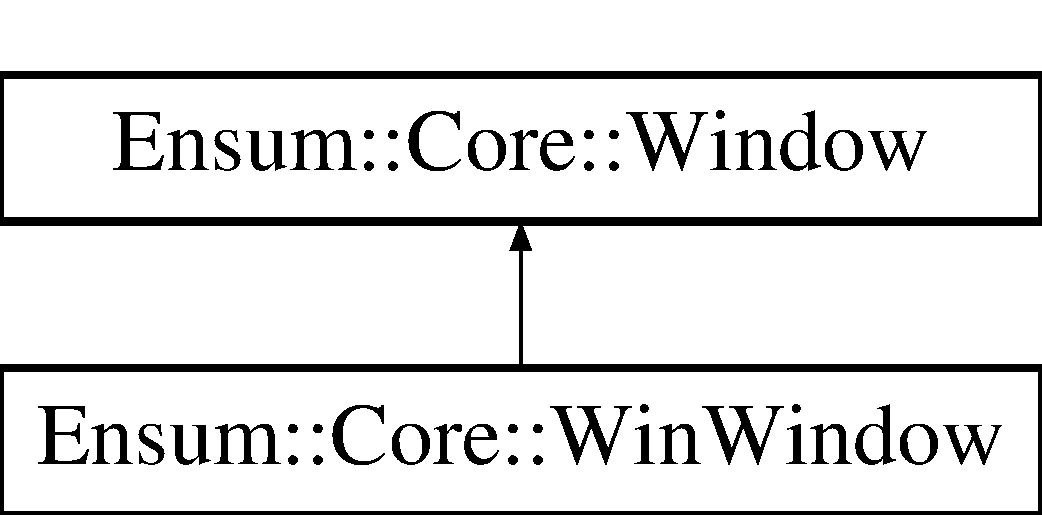
\includegraphics[height=2.000000cm]{class_ensum_1_1_core_1_1_window}
\end{center}
\end{figure}
\subsection*{Public Member Functions}
\begin{DoxyCompactItemize}
\item 
virtual const void \hyperlink{class_ensum_1_1_core_1_1_window_a43f467e7e5ea83f3a9b990b6edc2ec46}{Init} ()=0\hypertarget{class_ensum_1_1_core_1_1_window_a43f467e7e5ea83f3a9b990b6edc2ec46}{}\label{class_ensum_1_1_core_1_1_window_a43f467e7e5ea83f3a9b990b6edc2ec46}

\begin{DoxyCompactList}\small\item\em Initialization for the window. \end{DoxyCompactList}\item 
virtual const void \hyperlink{class_ensum_1_1_core_1_1_window_aeafece8bb46d29de1de3ddf092662195}{Start} ()=0\hypertarget{class_ensum_1_1_core_1_1_window_aeafece8bb46d29de1de3ddf092662195}{}\label{class_ensum_1_1_core_1_1_window_aeafece8bb46d29de1de3ddf092662195}

\begin{DoxyCompactList}\small\item\em Start the message loop. \end{DoxyCompactList}\item 
\hyperlink{class_ensum_1_1_input_1_1_input}{Input\+::\+Input} $\ast$ \hyperlink{class_ensum_1_1_core_1_1_window_af746ffdd0281b2722d162fbf96c3542b}{Get\+Input} ()\hypertarget{class_ensum_1_1_core_1_1_window_af746ffdd0281b2722d162fbf96c3542b}{}\label{class_ensum_1_1_core_1_1_window_af746ffdd0281b2722d162fbf96c3542b}

\begin{DoxyCompactList}\small\item\em Returns a pointer to the input. \end{DoxyCompactList}\end{DoxyCompactItemize}
\subsection*{Static Public Member Functions}
\begin{DoxyCompactItemize}
\item 
static \hyperlink{class_ensum_1_1_core_1_1_window}{Window} $\ast$ \hyperlink{class_ensum_1_1_core_1_1_window_af9478f4a6643763ba3be7a1a9fc98377}{Create\+Win} (\hyperlink{class_ensum_1_1_core_1_1_window}{Window} $\ast$window)\hypertarget{class_ensum_1_1_core_1_1_window_af9478f4a6643763ba3be7a1a9fc98377}{}\label{class_ensum_1_1_core_1_1_window_af9478f4a6643763ba3be7a1a9fc98377}

\begin{DoxyCompactList}\small\item\em Saves the given window and initializes it. \end{DoxyCompactList}\item 
static \hyperlink{class_ensum_1_1_core_1_1_window}{Window} $\ast$ \hyperlink{class_ensum_1_1_core_1_1_window_ada827fab647cc63b1c389f91f670bf18}{Get\+Instance} ()\hypertarget{class_ensum_1_1_core_1_1_window_ada827fab647cc63b1c389f91f670bf18}{}\label{class_ensum_1_1_core_1_1_window_ada827fab647cc63b1c389f91f670bf18}

\begin{DoxyCompactList}\small\item\em Returns a pointer to the window. \end{DoxyCompactList}\item 
static void \hyperlink{class_ensum_1_1_core_1_1_window_ac6e8b05158fca2587cdfe23dabf35baf}{Delete\+Instance} ()
\begin{DoxyCompactList}\small\item\em Deletes the window. \end{DoxyCompactList}\end{DoxyCompactItemize}
\subsection*{Public Attributes}
\begin{DoxyCompactItemize}
\item 
\hyperlink{class_ensum_1_1_utils_1_1_event}{Utils\+::\+Event}$<$ const void()$>$ {\bfseries Frame\+Start}\hypertarget{class_ensum_1_1_core_1_1_window_ad122b1a7fa3fdfcb351abbad2252dfe2}{}\label{class_ensum_1_1_core_1_1_window_ad122b1a7fa3fdfcb351abbad2252dfe2}

\end{DoxyCompactItemize}
\subsection*{Protected Member Functions}
\begin{DoxyCompactItemize}
\item 
virtual const void \hyperlink{class_ensum_1_1_core_1_1_window_a58af9c1b06e0fe12820f584f4638ae15}{Frame} ()=0
\begin{DoxyCompactList}\small\item\em The frame function. \end{DoxyCompactList}\end{DoxyCompactItemize}
\subsection*{Protected Attributes}
\begin{DoxyCompactItemize}
\item 
\hyperlink{class_ensum_1_1_core_1_1_timer}{Timer} $\ast$ {\bfseries \+\_\+timer}\hypertarget{class_ensum_1_1_core_1_1_window_aa27d25534350ec8e46cf2eae67c82ea5}{}\label{class_ensum_1_1_core_1_1_window_aa27d25534350ec8e46cf2eae67c82ea5}

\item 
\hyperlink{class_ensum_1_1_input_1_1_input}{Input\+::\+Input} $\ast$ {\bfseries \+\_\+input}\hypertarget{class_ensum_1_1_core_1_1_window_a6b2925a490f7a5a2417059660713bc19}{}\label{class_ensum_1_1_core_1_1_window_a6b2925a490f7a5a2417059660713bc19}

\end{DoxyCompactItemize}
\subsection*{Static Protected Attributes}
\begin{DoxyCompactItemize}
\item 
static \hyperlink{class_ensum_1_1_core_1_1_window}{Window} $\ast$ {\bfseries \+\_\+instance}\hypertarget{class_ensum_1_1_core_1_1_window_aa4ca94e77186512ab2949dd6c7e850e6}{}\label{class_ensum_1_1_core_1_1_window_aa4ca94e77186512ab2949dd6c7e850e6}

\end{DoxyCompactItemize}


\subsection{Detailed Description}
Fully abstract class for interfacting with the actual window. 

\subsection{Member Function Documentation}
\index{Ensum\+::\+Core\+::\+Window@{Ensum\+::\+Core\+::\+Window}!Delete\+Instance@{Delete\+Instance}}
\index{Delete\+Instance@{Delete\+Instance}!Ensum\+::\+Core\+::\+Window@{Ensum\+::\+Core\+::\+Window}}
\subsubsection[{\texorpdfstring{Delete\+Instance()}{DeleteInstance()}}]{\setlength{\rightskip}{0pt plus 5cm}static void Ensum\+::\+Core\+::\+Window\+::\+Delete\+Instance (
\begin{DoxyParamCaption}
{}
\end{DoxyParamCaption}
)\hspace{0.3cm}{\ttfamily [static]}}\hypertarget{class_ensum_1_1_core_1_1_window_ac6e8b05158fca2587cdfe23dabf35baf}{}\label{class_ensum_1_1_core_1_1_window_ac6e8b05158fca2587cdfe23dabf35baf}


Deletes the window. 

This also deletes all members \index{Ensum\+::\+Core\+::\+Window@{Ensum\+::\+Core\+::\+Window}!Frame@{Frame}}
\index{Frame@{Frame}!Ensum\+::\+Core\+::\+Window@{Ensum\+::\+Core\+::\+Window}}
\subsubsection[{\texorpdfstring{Frame()=0}{Frame()=0}}]{\setlength{\rightskip}{0pt plus 5cm}virtual const void Ensum\+::\+Core\+::\+Window\+::\+Frame (
\begin{DoxyParamCaption}
{}
\end{DoxyParamCaption}
)\hspace{0.3cm}{\ttfamily [protected]}, {\ttfamily [pure virtual]}}\hypertarget{class_ensum_1_1_core_1_1_window_a58af9c1b06e0fe12820f584f4638ae15}{}\label{class_ensum_1_1_core_1_1_window_a58af9c1b06e0fe12820f584f4638ae15}


The frame function. 

Put the gamelogic here. 

Implemented in \hyperlink{class_ensum_1_1_core_1_1_win_window_a3e828ccbc90f0d6ed81c2320277561e6}{Ensum\+::\+Core\+::\+Win\+Window}.



The documentation for this class was generated from the following file\+:\begin{DoxyCompactItemize}
\item 
Includes/\+Ensum\+\_\+core/Window.\+h\end{DoxyCompactItemize}

\hypertarget{class_ensum_1_1_core_1_1_win_window}{}\section{Ensum\+:\+:Core\+:\+:Win\+Window Class Reference}
\label{class_ensum_1_1_core_1_1_win_window}\index{Ensum\+::\+Core\+::\+Win\+Window@{Ensum\+::\+Core\+::\+Win\+Window}}


Windows specific window.  




{\ttfamily \#include $<$Windows\+Window.\+h$>$}

Inheritance diagram for Ensum\+:\+:Core\+:\+:Win\+Window\+:\begin{figure}[H]
\begin{center}
\leavevmode
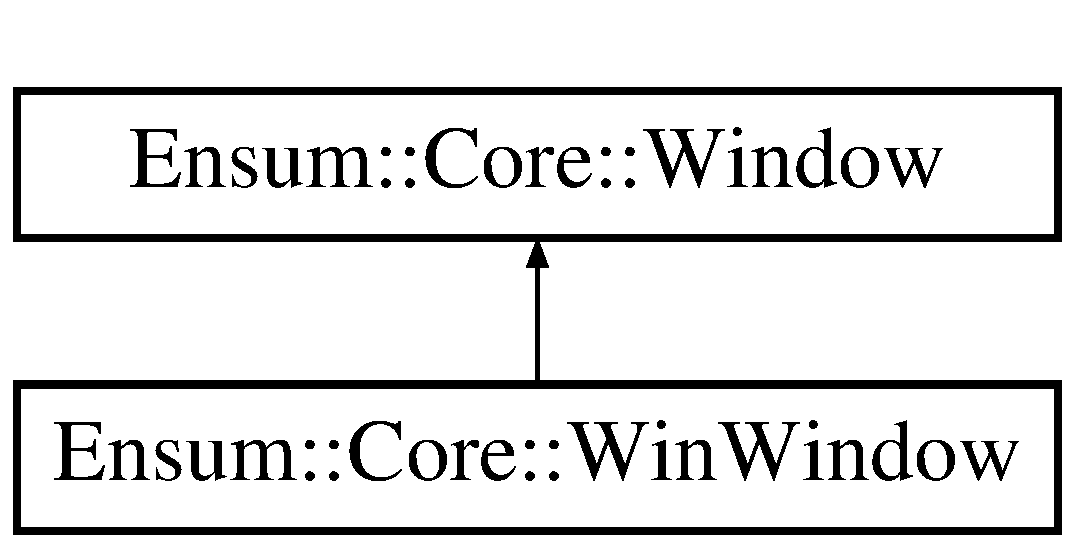
\includegraphics[height=2.000000cm]{class_ensum_1_1_core_1_1_win_window}
\end{center}
\end{figure}
\subsection*{Public Member Functions}
\begin{DoxyCompactItemize}
\item 
virtual const void \hyperlink{class_ensum_1_1_core_1_1_win_window_afb59ce364f98918b2b17653cbfc39ead}{Init} ()\hypertarget{class_ensum_1_1_core_1_1_win_window_afb59ce364f98918b2b17653cbfc39ead}{}\label{class_ensum_1_1_core_1_1_win_window_afb59ce364f98918b2b17653cbfc39ead}

\begin{DoxyCompactList}\small\item\em Initialization for the window. \end{DoxyCompactList}\item 
virtual const void \hyperlink{class_ensum_1_1_core_1_1_win_window_a1c316902d186c3d685210237e3438745}{Start} ()\hypertarget{class_ensum_1_1_core_1_1_win_window_a1c316902d186c3d685210237e3438745}{}\label{class_ensum_1_1_core_1_1_win_window_a1c316902d186c3d685210237e3438745}

\begin{DoxyCompactList}\small\item\em Start the message loop. \end{DoxyCompactList}\end{DoxyCompactItemize}
\subsection*{Protected Member Functions}
\begin{DoxyCompactItemize}
\item 
virtual const void \hyperlink{class_ensum_1_1_core_1_1_win_window_a3e828ccbc90f0d6ed81c2320277561e6}{Frame} ()
\begin{DoxyCompactList}\small\item\em The frame function. \end{DoxyCompactList}\end{DoxyCompactItemize}
\subsection*{Protected Attributes}
\begin{DoxyCompactItemize}
\item 
H\+I\+N\+S\+T\+A\+N\+CE {\bfseries \+\_\+h\+Inst}\hypertarget{class_ensum_1_1_core_1_1_win_window_a19562456a0e7d38dc67b673ad8c0a9ea}{}\label{class_ensum_1_1_core_1_1_win_window_a19562456a0e7d38dc67b673ad8c0a9ea}

\item 
H\+W\+ND {\bfseries \+\_\+h\+Wnd}\hypertarget{class_ensum_1_1_core_1_1_win_window_af0bdb075823585bf3f99895ab4dcfffa}{}\label{class_ensum_1_1_core_1_1_win_window_af0bdb075823585bf3f99895ab4dcfffa}

\item 
D\+W\+O\+RD {\bfseries \+\_\+style}\hypertarget{class_ensum_1_1_core_1_1_win_window_af2bbdea21686b0d5a38bd3c85bc8f7db}{}\label{class_ensum_1_1_core_1_1_win_window_af2bbdea21686b0d5a38bd3c85bc8f7db}

\item 
L\+P\+W\+S\+TR {\bfseries \+\_\+wnd\+Caption}\hypertarget{class_ensum_1_1_core_1_1_win_window_a75879298465e6dab7671f0028489f82a}{}\label{class_ensum_1_1_core_1_1_win_window_a75879298465e6dab7671f0028489f82a}

\item 
bool {\bfseries \+\_\+running}\hypertarget{class_ensum_1_1_core_1_1_win_window_a11e86f63066c9cb730c152b23f2e5378}{}\label{class_ensum_1_1_core_1_1_win_window_a11e86f63066c9cb730c152b23f2e5378}

\end{DoxyCompactItemize}
\subsection*{Additional Inherited Members}


\subsection{Detailed Description}
Windows specific window. 

\subsection{Member Function Documentation}
\index{Ensum\+::\+Core\+::\+Win\+Window@{Ensum\+::\+Core\+::\+Win\+Window}!Frame@{Frame}}
\index{Frame@{Frame}!Ensum\+::\+Core\+::\+Win\+Window@{Ensum\+::\+Core\+::\+Win\+Window}}
\subsubsection[{\texorpdfstring{Frame()}{Frame()}}]{\setlength{\rightskip}{0pt plus 5cm}virtual const void Ensum\+::\+Core\+::\+Win\+Window\+::\+Frame (
\begin{DoxyParamCaption}
{}
\end{DoxyParamCaption}
)\hspace{0.3cm}{\ttfamily [protected]}, {\ttfamily [virtual]}}\hypertarget{class_ensum_1_1_core_1_1_win_window_a3e828ccbc90f0d6ed81c2320277561e6}{}\label{class_ensum_1_1_core_1_1_win_window_a3e828ccbc90f0d6ed81c2320277561e6}


The frame function. 

Put the gamelogic here. 

Implements \hyperlink{class_ensum_1_1_core_1_1_window_a58af9c1b06e0fe12820f584f4638ae15}{Ensum\+::\+Core\+::\+Window}.



The documentation for this class was generated from the following file\+:\begin{DoxyCompactItemize}
\item 
Includes/\+Ensum\+\_\+core/Windows\+Window.\+h\end{DoxyCompactItemize}

%--- End generated contents ---

% Index
\backmatter
\newpage
\phantomsection
\clearemptydoublepage
\addcontentsline{toc}{chapter}{Index}
\printindex

\end{document}
